\documentclass[hyperref=colorlinks]{beamer}
\mode<presentation>
\usetheme{iclpt}
\setbeamertemplate{navigation symbols}{}
\setbeamertemplate{headline}{
\begin{beamercolorbox}[leftskip=.2cm,rightskip=.2cm,topskip=.2cm,ht=1.1cm,dp=0.1cm,wd=\textwidth]{institute in head/foot}
  
\includegraphics[height=1cm]{icl.pdf}
  \hfill
  
\includegraphics[height=1cm]{../Pics/CMS-Color.pdf}
\end{beamercolorbox}
}
\setbeamertemplate{footline}{
\begin{beamercolorbox}[ht=.55cm,dp=0.4cm,wd=\textwidth,leftskip=.3cm]{author in head/foot}%
  \begin{minipage}[c]{5cm}%
    \usebeamerfont{author in head/foot}
    \insertshortauthor 
    \insertshorttitle
    \end{minipage}\hfill%
  \insertframenumber{} / \pageref{lastframe}
  \hfill
  \begin{minipage}{6cm}
    \hfill
  \end{minipage}
\end{beamercolorbox}%
}

\usepackage{color}
\usepackage{tabularx,colortbl}
\usepackage{graphicx}
\usepackage{pdfpages}
\usepackage{feynmp}
\usepackage{tikz}
\usetikzlibrary{calc, shapes, backgrounds,arrows,positioning}
\DeclareGraphicsRule{*}{mps}{*}{}

\title{\vspace{-0.2cm} VBF Higgs to Invisible}
\subtitle{HIG-14-038, AN-14-243\vspace{-0.7cm}}
\author[]{}%\underline{P. Dunne}} % A.M. Magnan and A. Nikitenko Joao Pela with \\ R. Aggleton, J. Brooke: Bristol \\ C.Asawangtrakuldee, Q.Li: Peking \\ P. Srimanobhas: Chulalongkorn \\ S. Kumar, K. Mazumdar: Mumbai}
\titlegraphic{
  \vspace{-0.7cm}
  %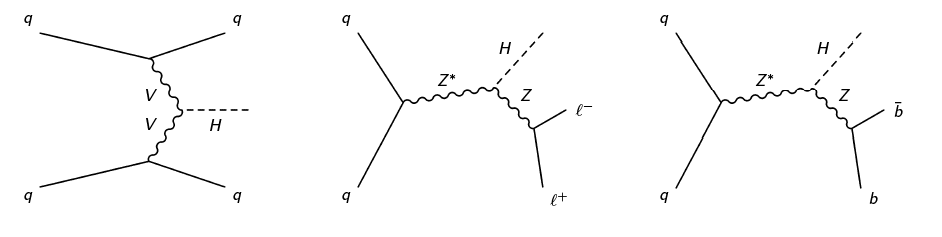
\includegraphics[width=\textwidth]{TalkPics/invcomb021213/feyndiags}
  %% \begin{fmfgraph*}(100,70)
  %%         \fmfleft{i1,i2}
  %%         \fmfright{o1,o2,o3}
  %%         \fmf{fermion}{i1,v1,o1}
  %%         \fmf{fermion}{i2,v2,o3}
  %%         \fmf{phantom,tension=4/5}{v1,v2}
  %%         \fmffreeze
  %%         \fmf{photon,label=$W,,Z$}{v1,v3}
  %%         \fmf{photon,label=$W,,Z$}{v2,v3}
  %%         \fmf{dashes}{v3,o2}
  %%         \fmflabel{$q$}{i1}
  %%         \fmflabel{$q$}{i2}
  %%         \fmflabel{$q$}{o1}
  %%         \fmflabel{$q$}{o3}
  %%         \fmflabel{$H$}{o2}
  %%       \end{fmfgraph*}
}
\date{}
\begin{document}
\begin{fmffile}{higgsexoupdatefeyndiags}
\tikzstyle{every picture}+=[remember picture]

%TITLE PAGE
\section{Title}
\begin{frame}
  \titlepage
  
\end{frame}

\begin{frame}
  \frametitle{Overview}
  \begin{block}{Reminder}
    \begin{itemize}
    \item First signal MC comparisons between run 1 and run 2 performed
    \item Jet $\eta$ ``ears'' problem seen
    \item[-] to be improved in CMSSW\_7\_4\_2
    \end{itemize}
  \end{block}
  \begin{block}{New Today}
    \begin{itemize}
    \item Some technical problems with dcache necessitated rerunning QCD ntuples
    \item Now complete: first control plots today
    \item Have also remade DM interpretation plot with parked result
    \end{itemize}
    \end{block}
\end{frame}

\begin{frame}
  \frametitle{QCD and signal comparison: run 1 vs run 2}
  \begin{block}{}
    \begin{itemize}
    \item Run2 QCD is inclusive PU20B25
    \item As in run 1 very little QCD MC in signal region so start from loose region:
      $\eta_{j1} \cdot \eta_{j2}<0,\, \eta_{j1}<4.7,\, \eta_{j2}<4.7,$
      $p_{T}^{\text{j1}}>50 \,\text{GeV},\,p_{T}^{\text{j2}}>40\,\text{GeV},$
      $\Delta\eta_{jj}>3.6,\, M_{jj}>800\,\text{GeV},$
      $MET>90\,\text{GeV},$
      $METsig>3.$
    \item Data/Bkg is Run 2 QCD inc/Run 1 QCD inc
    \item As last time trigger weighting etc. as in parked analysis
    \item All distributions normalised to 1
    \end{itemize}
  \end{block}
\end{frame}

\begin{frame}
  \frametitle{Signal comparison: run 1 vs run 2: Jet $p_{T}$}
  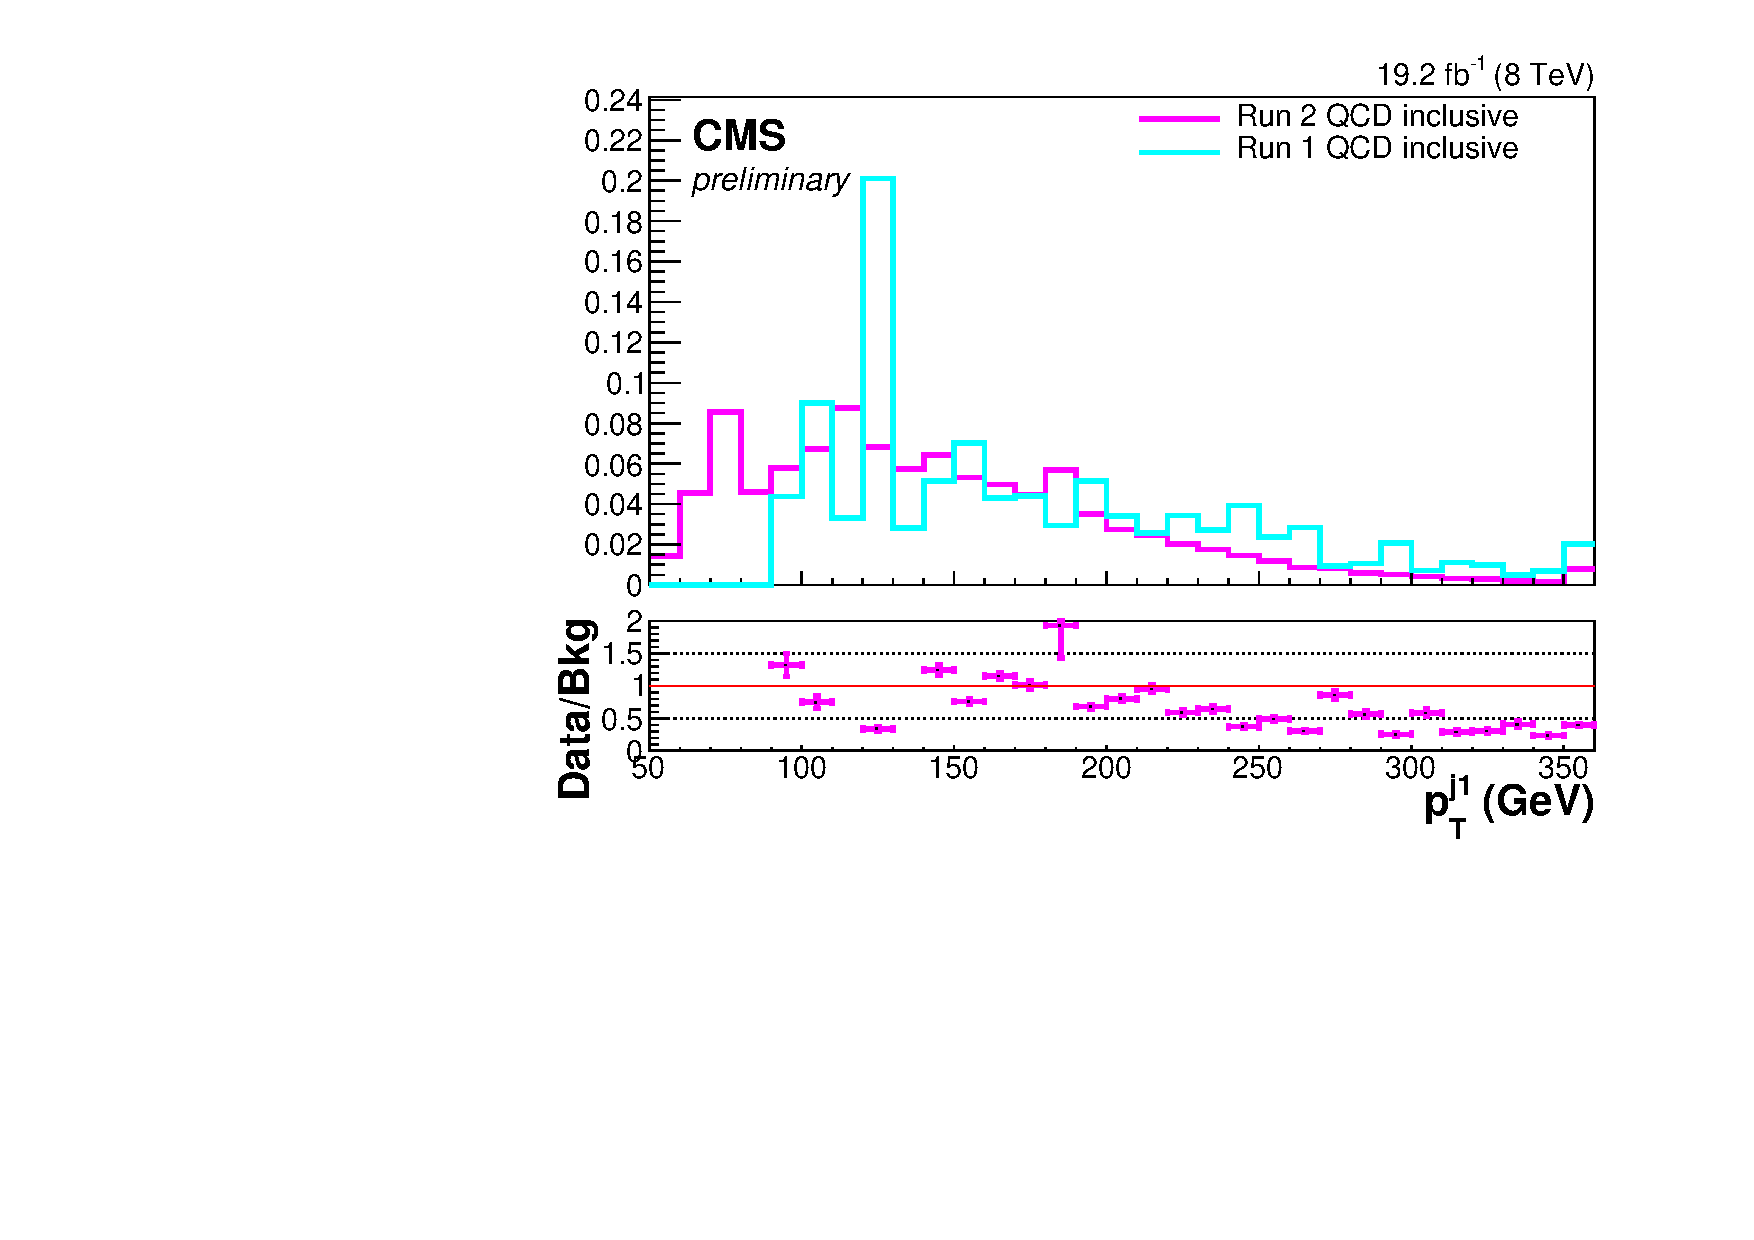
\includegraphics[width=.5\textwidth]{TalkPics/dmandqcd010615/qcdplots010615/nunu_norm_jet1_pt.pdf}
  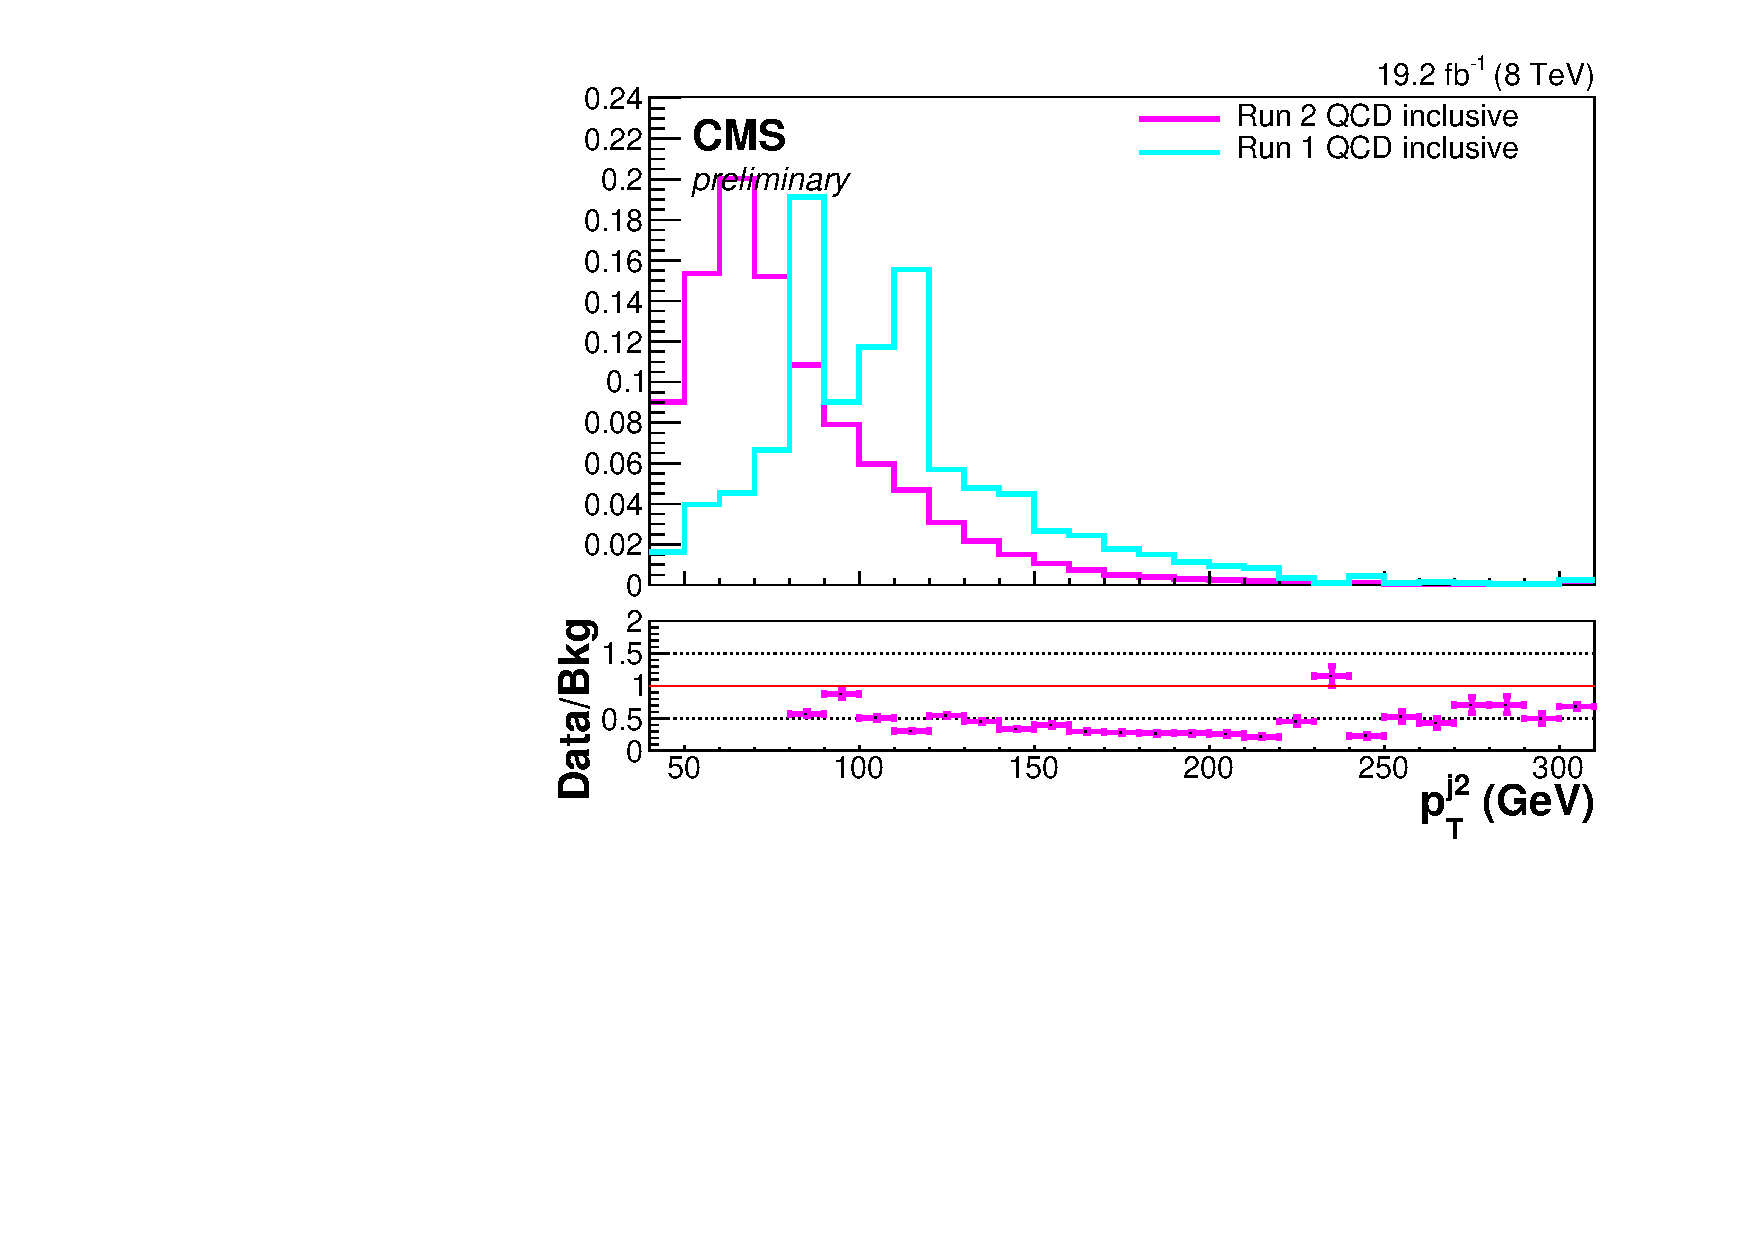
\includegraphics[width=.5\textwidth]{TalkPics/dmandqcd010615/qcdplots010615/nunu_norm_jet2_pt.pdf}
  \begin{block}{}
    \begin{itemize}
    \item[-] Low statistics in run 1 MC but appears higher in pt
    \end{itemize}
  \end{block}
\end{frame}

\begin{frame}
  \frametitle{Signal comparison: run 1 vs run 2: Jet $\eta$}
  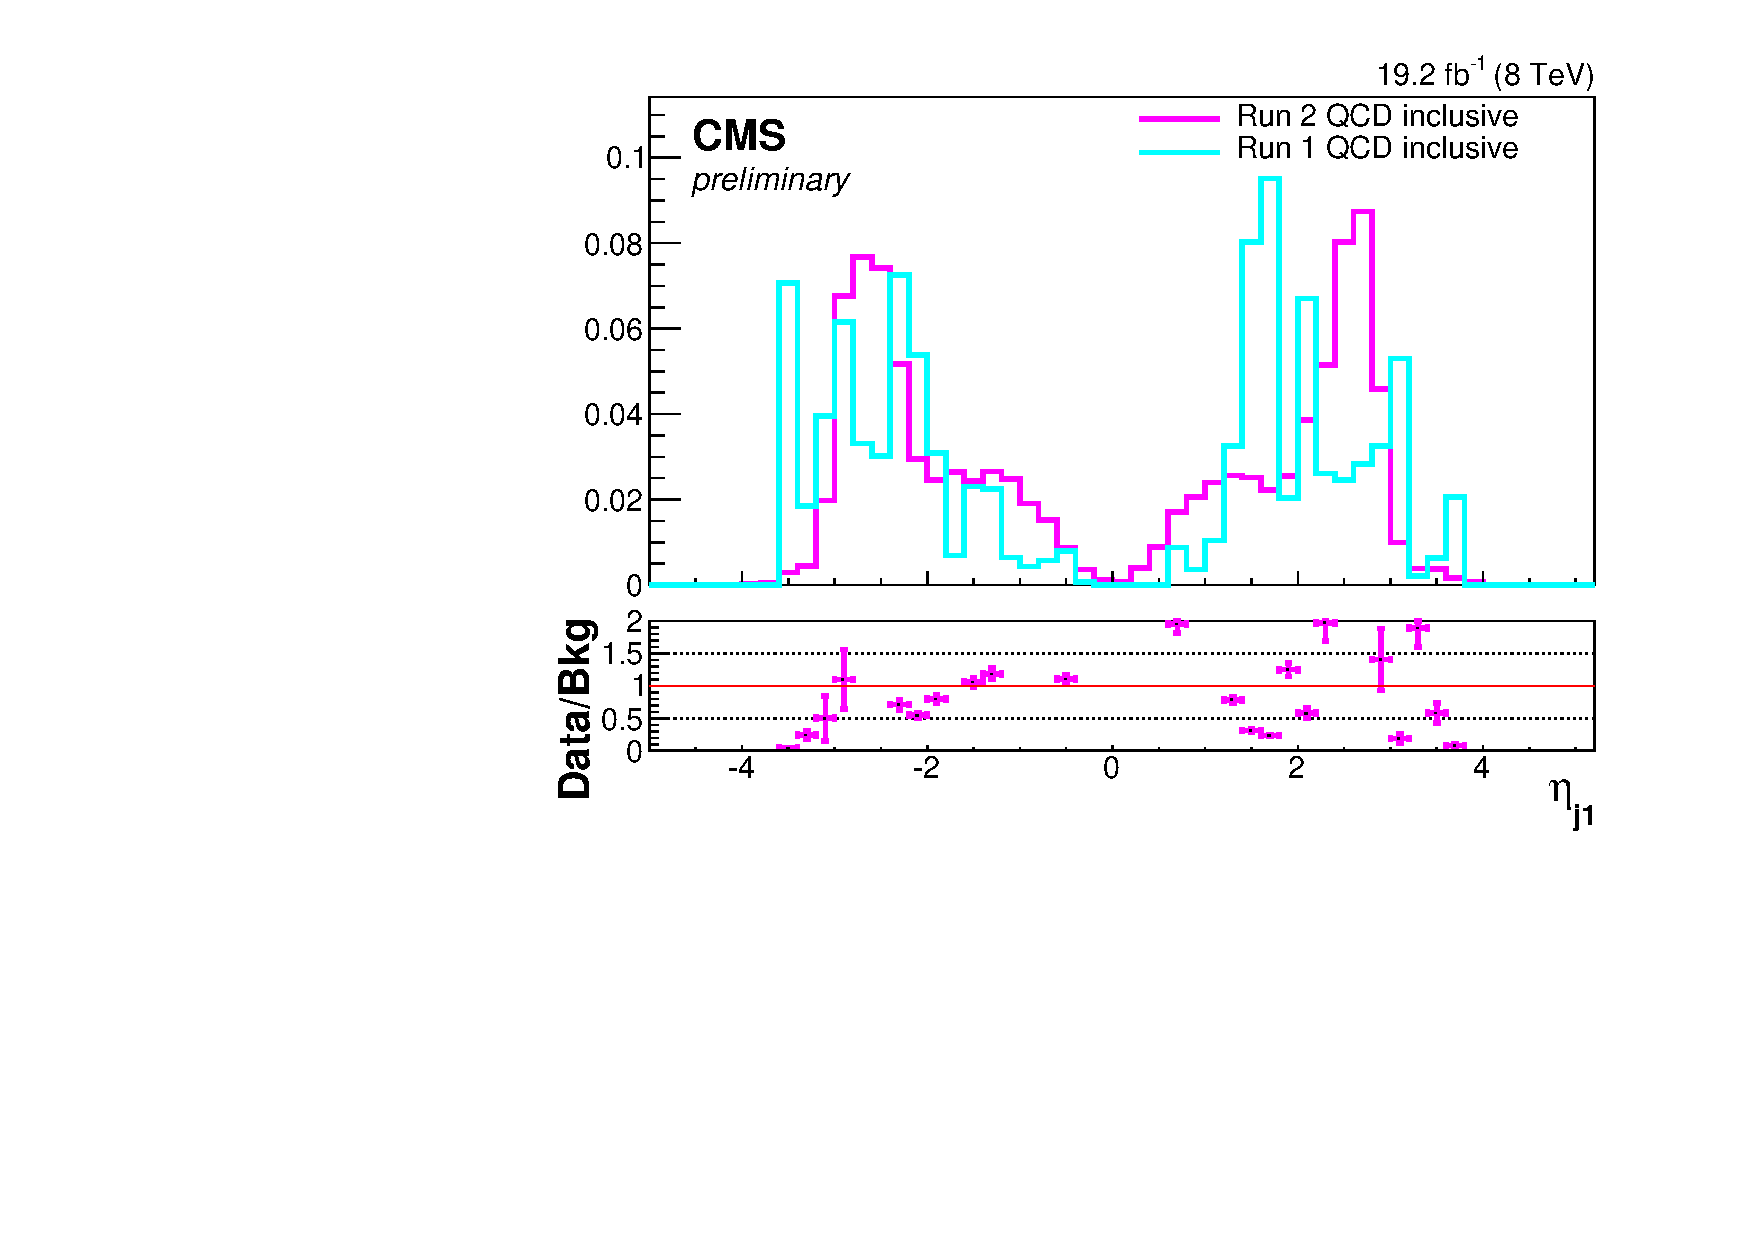
\includegraphics[width=.5\textwidth]{TalkPics/dmandqcd010615/qcdplots010615/nunu_norm_jet1_eta.pdf}
  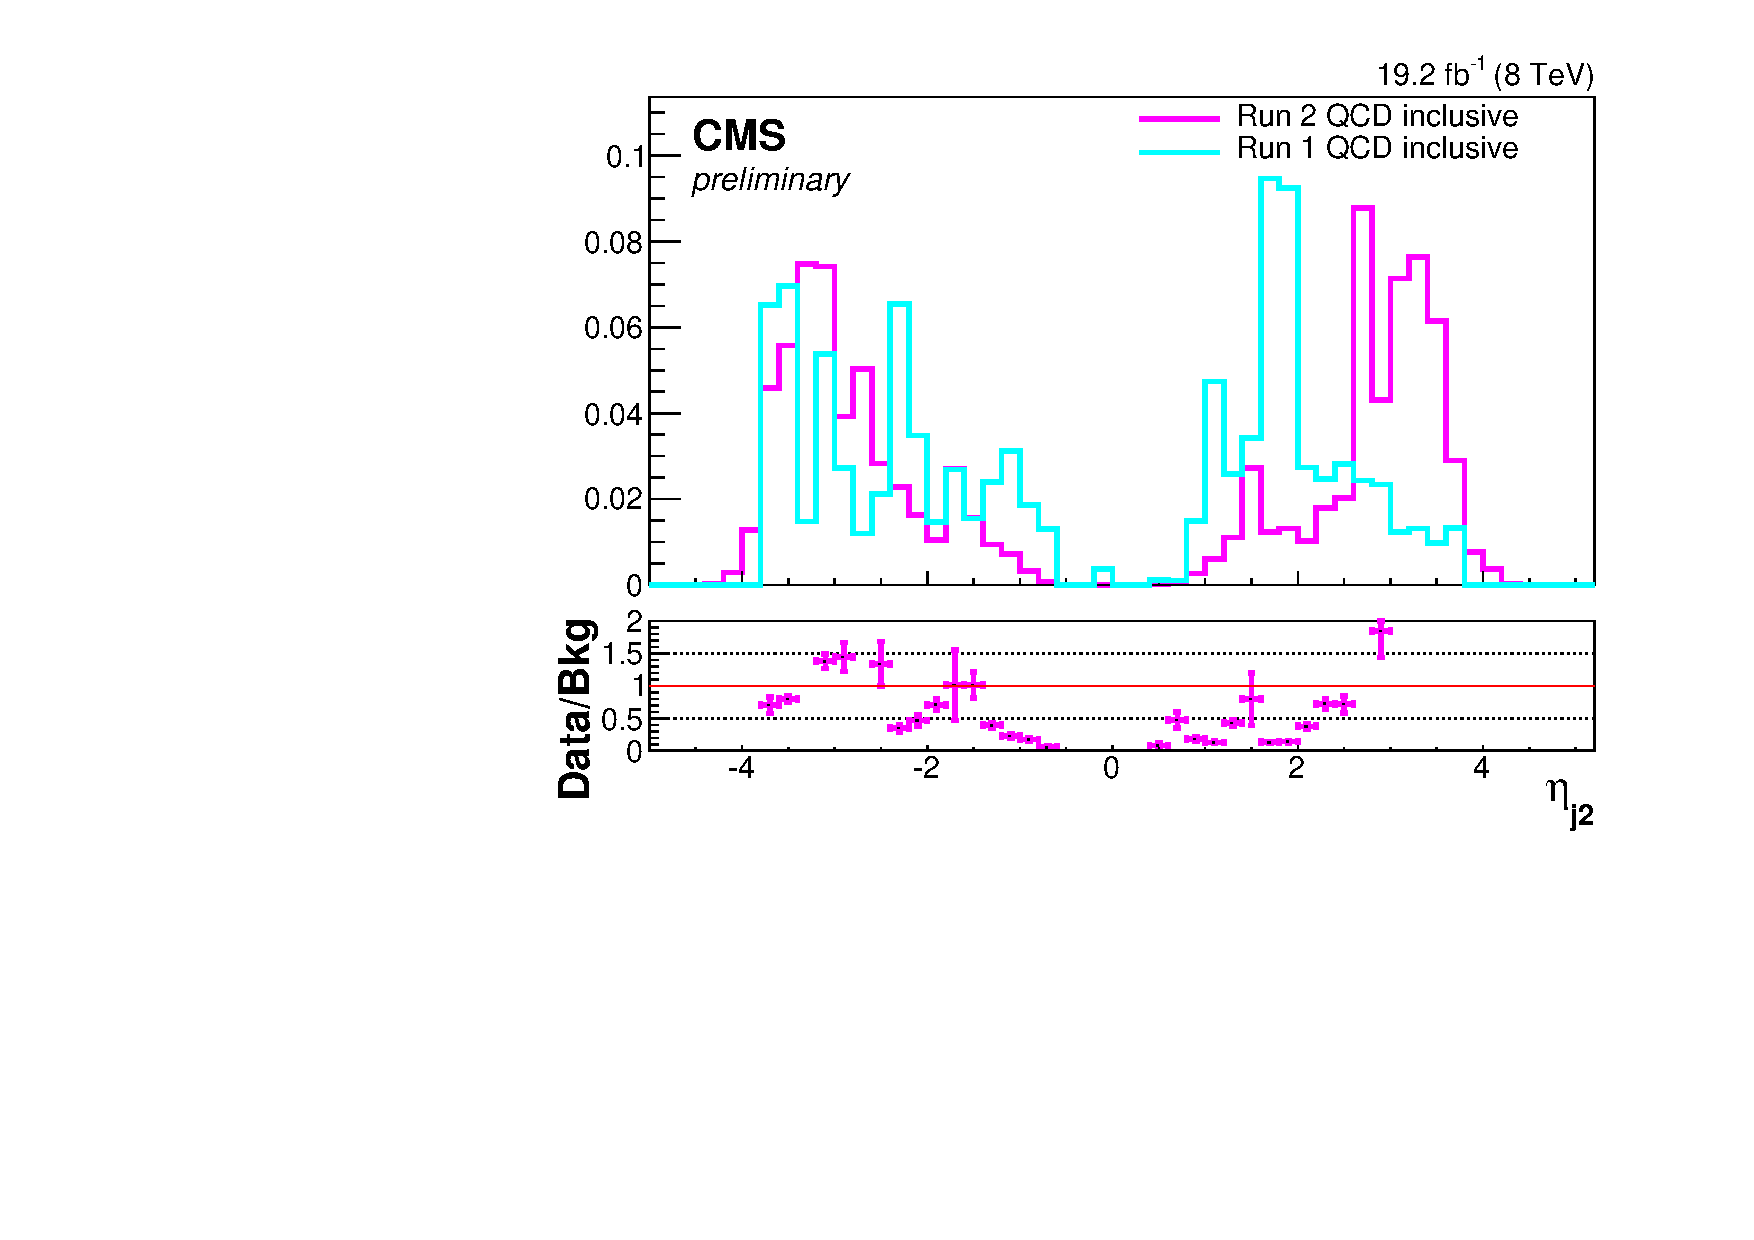
\includegraphics[width=.5\textwidth]{TalkPics/dmandqcd010615/qcdplots010615/nunu_norm_jet2_eta.pdf}
  \begin{block}{}
    \begin{itemize}
    \item Jet 1 has ears from 2.5-3 as well
    \item Jet 2 has a lot of events in the HF
    \end{itemize}
  \end{block}
\end{frame}

\begin{frame}
  \frametitle{Signal comparison: run 1 vs run 2: Jet $\phi$}
  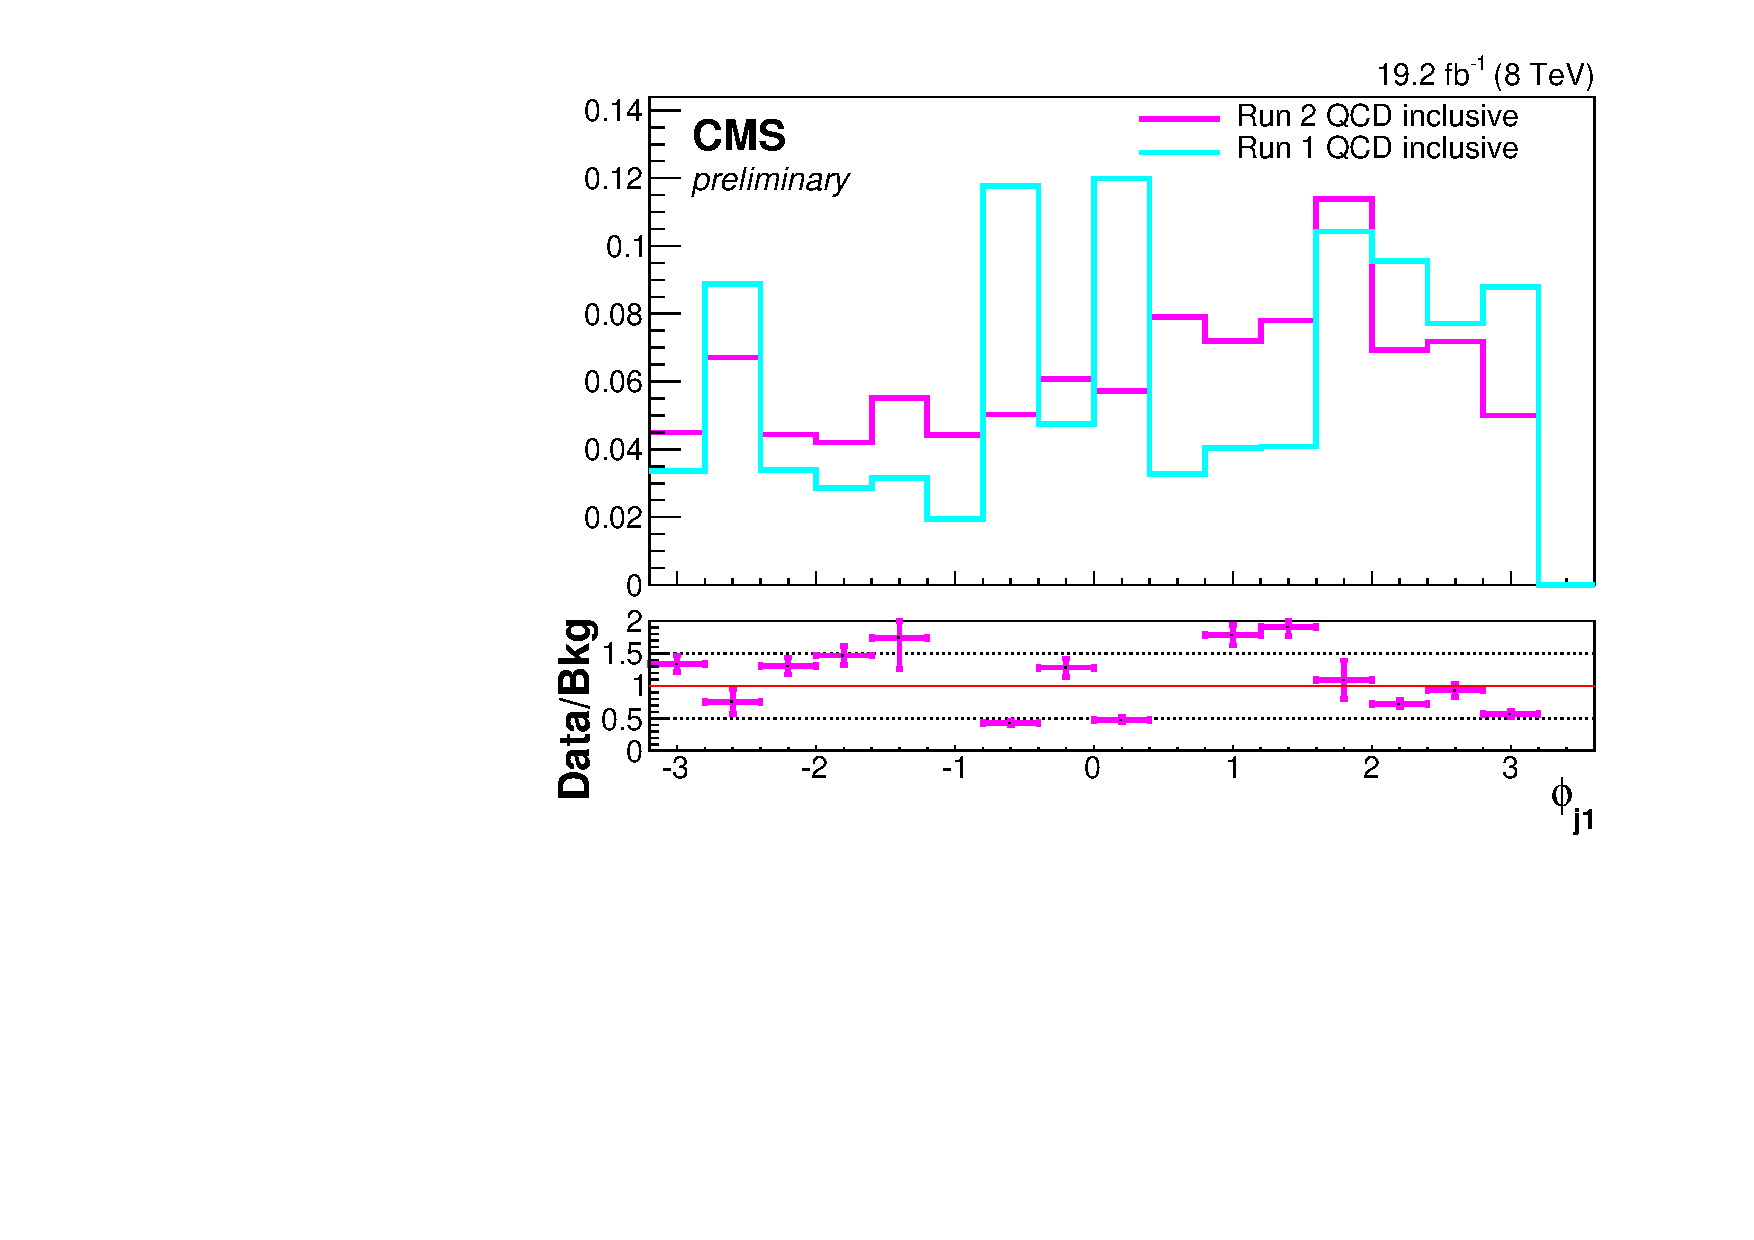
\includegraphics[width=.5\textwidth]{TalkPics/dmandqcd010615/qcdplots010615/nunu_norm_jet1_phi.pdf}
  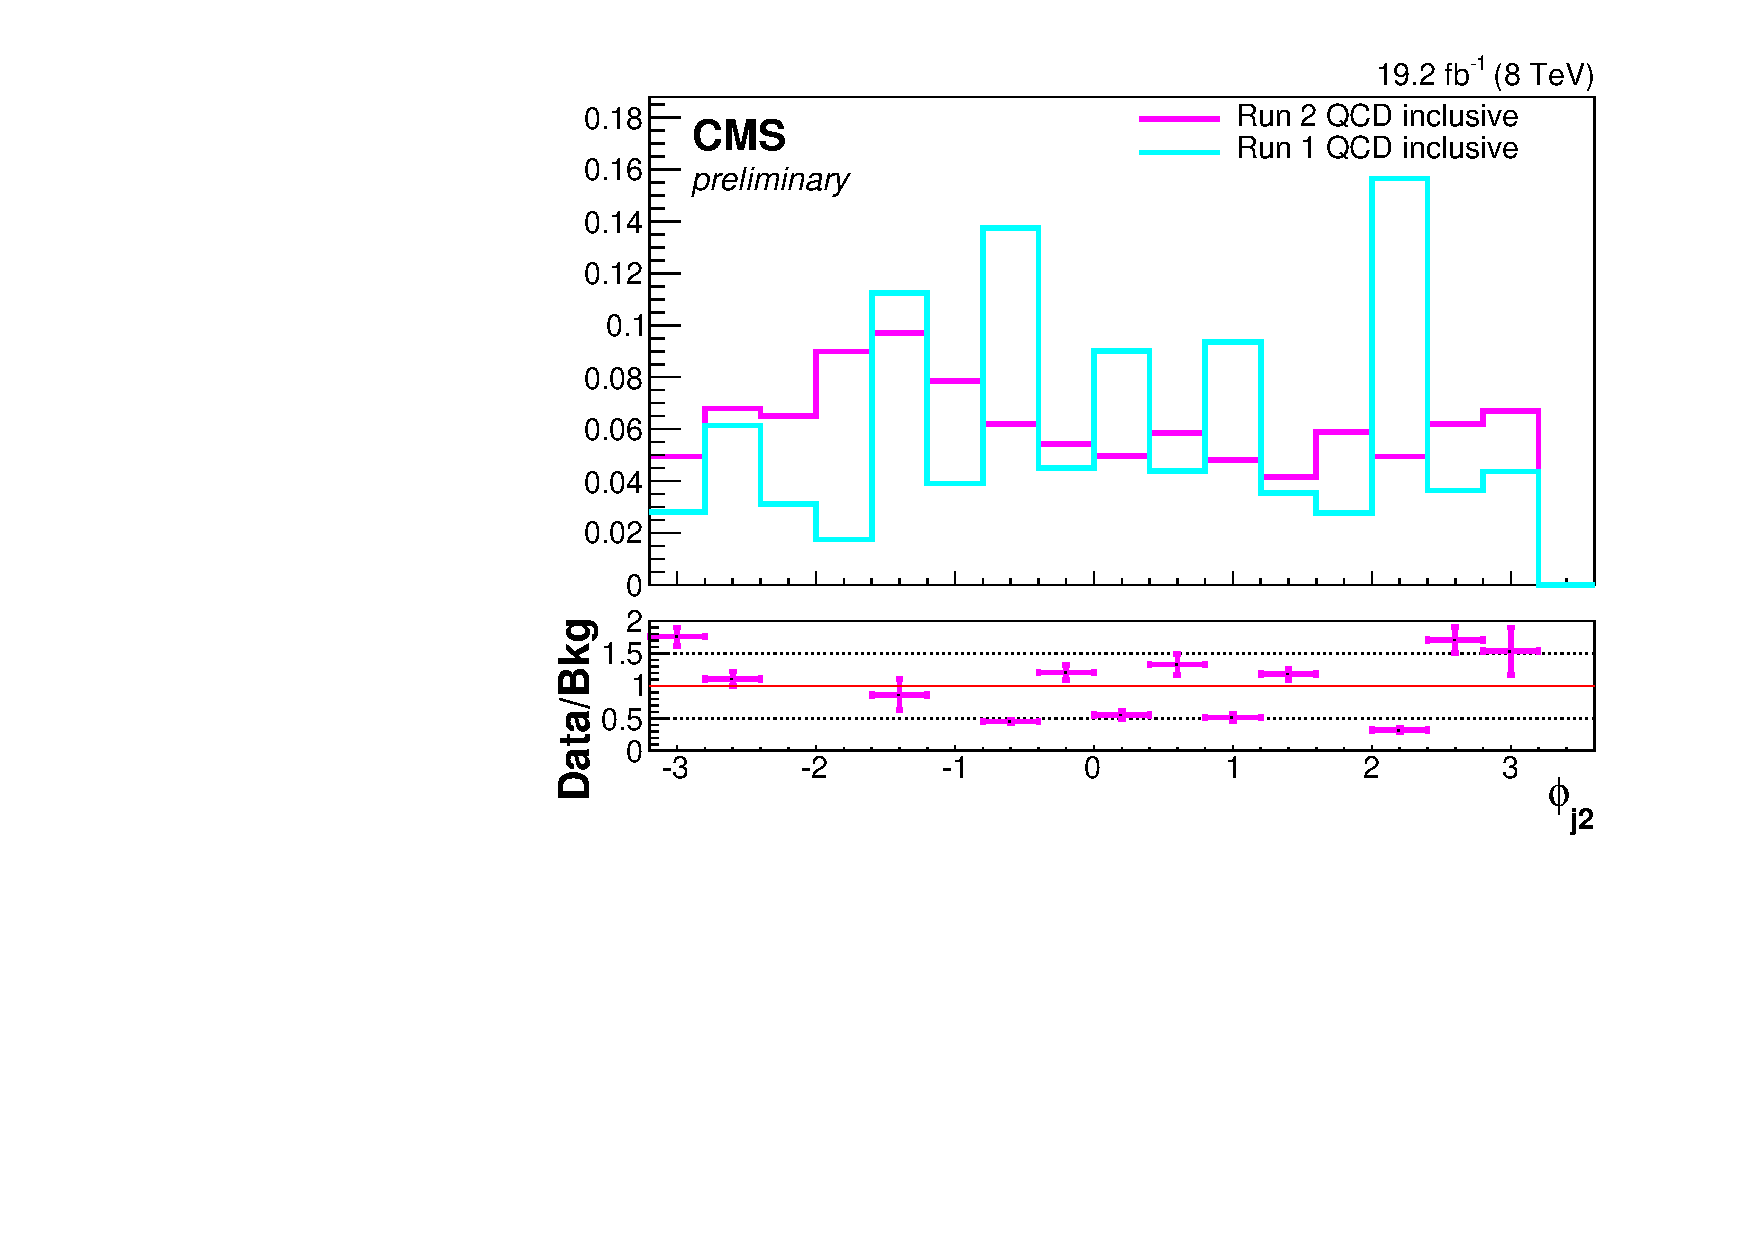
\includegraphics[width=.5\textwidth]{TalkPics/dmandqcd010615/qcdplots010615/nunu_norm_jet2_phi.pdf}
  \begin{block}{}
    \begin{itemize}
    \item $\phi$ distributions look similar within stat error
    \end{itemize}
  \end{block}
\end{frame}

\begin{frame}
  \frametitle{Signal comparison: run 1 vs run 2: Met}
  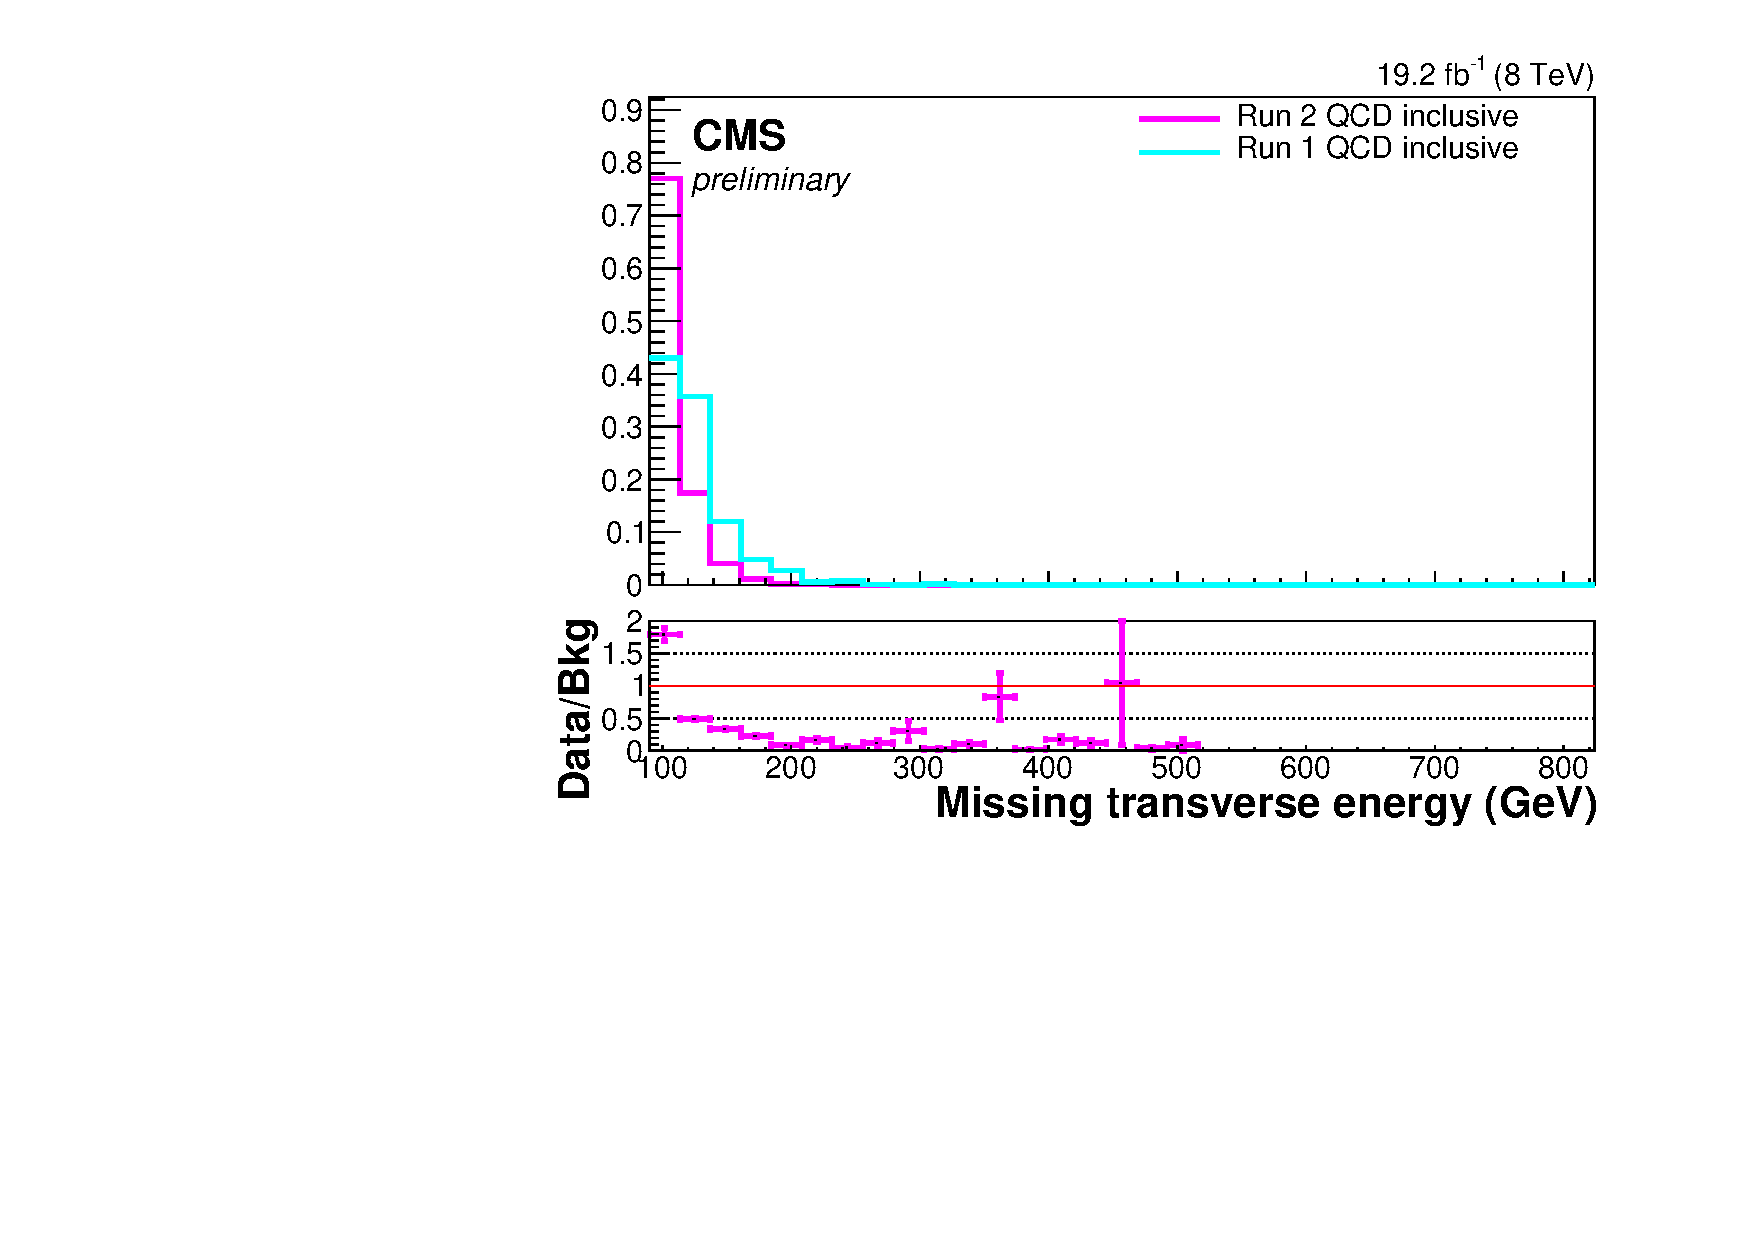
\includegraphics[width=.5\textwidth]{TalkPics/dmandqcd010615/qcdplots010615/nunu_norm_metnomuons.pdf}
  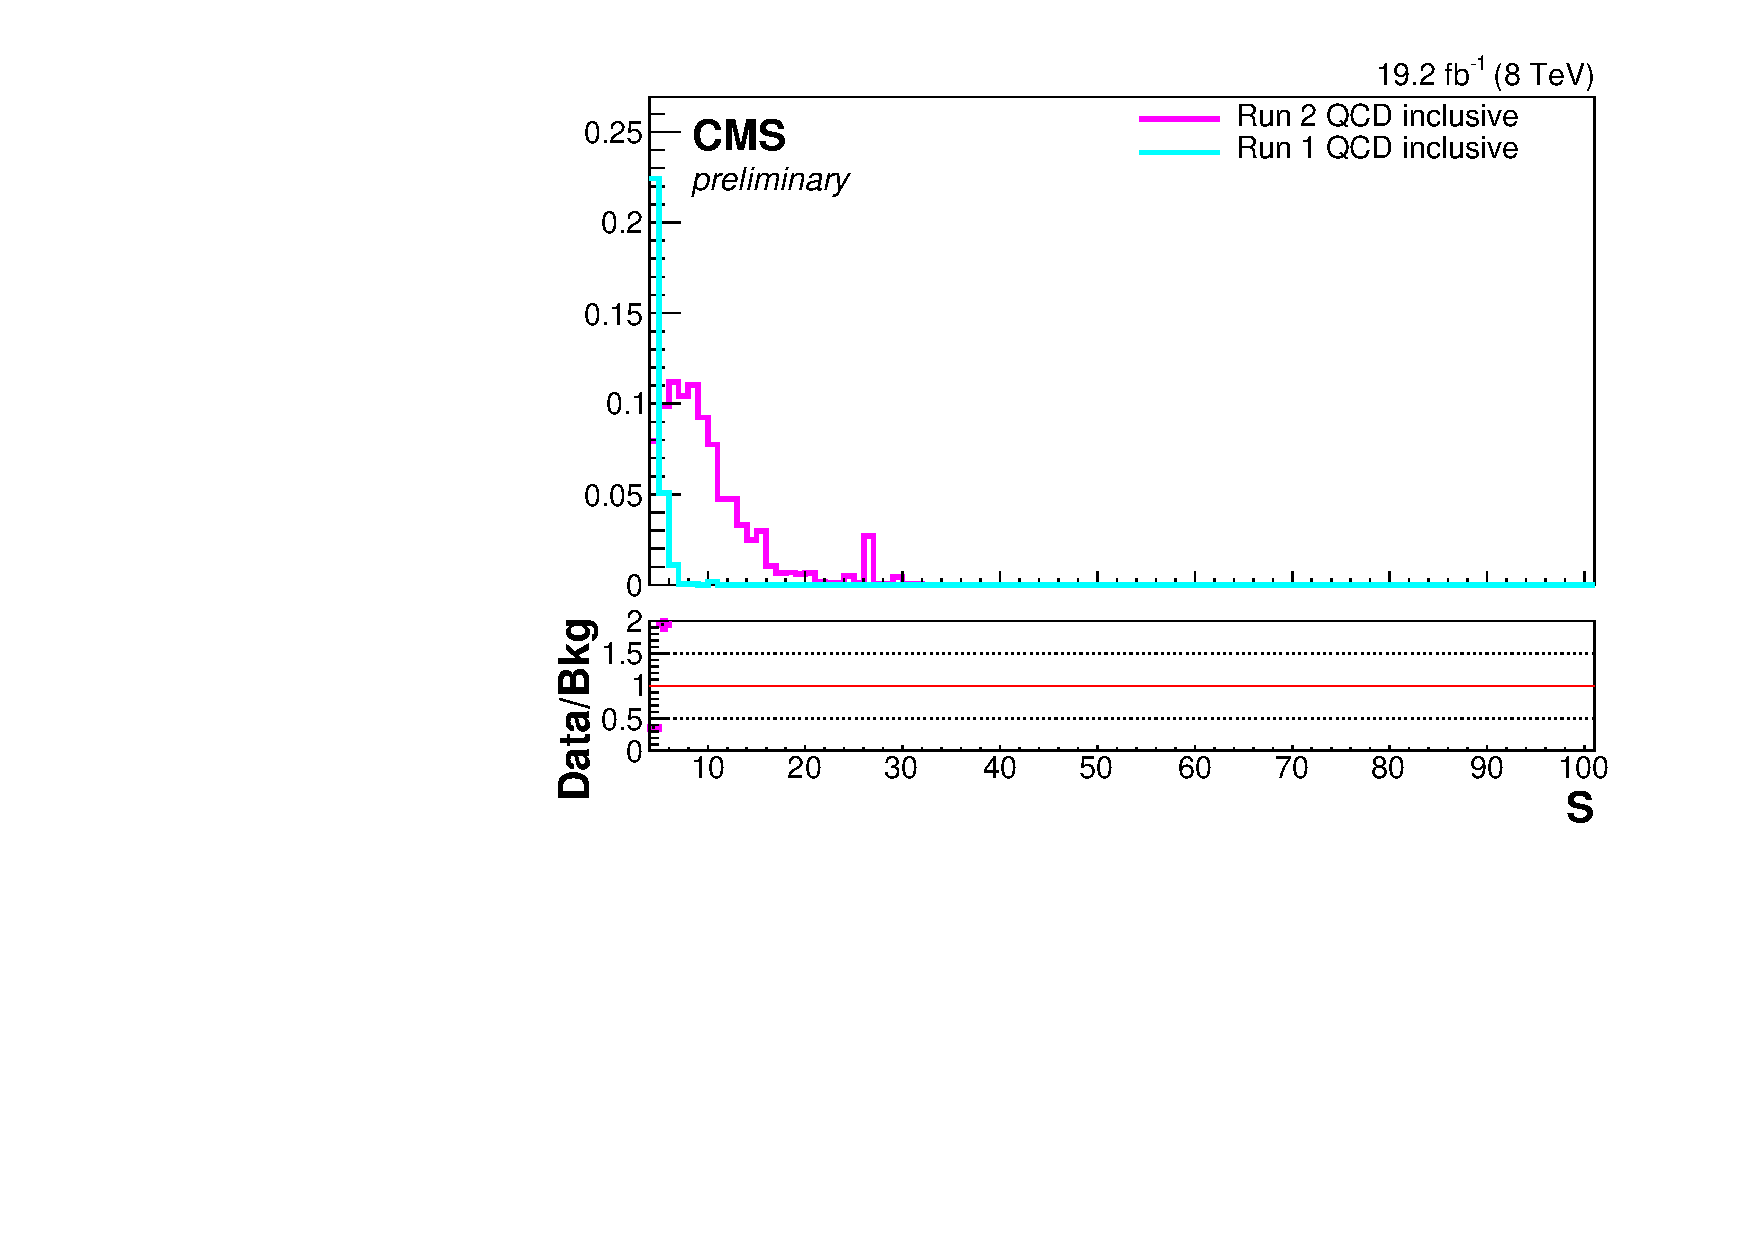
\includegraphics[width=.5\textwidth]{TalkPics/dmandqcd010615/qcdplots010615/nunu_norm_metnomu_significance.pdf}
  \begin{block}{}
    \begin{itemize}
    \item QCD Met lower for run 2 although no fake met in inclusive samples
    \item Met significance is a different variable in miniAOD to the one we used in run 1
    \end{itemize}
  \end{block}
\end{frame}

\begin{frame}
  \frametitle{Signal comparison: run 1 vs run 2: $\Delta\phi$ variables}
  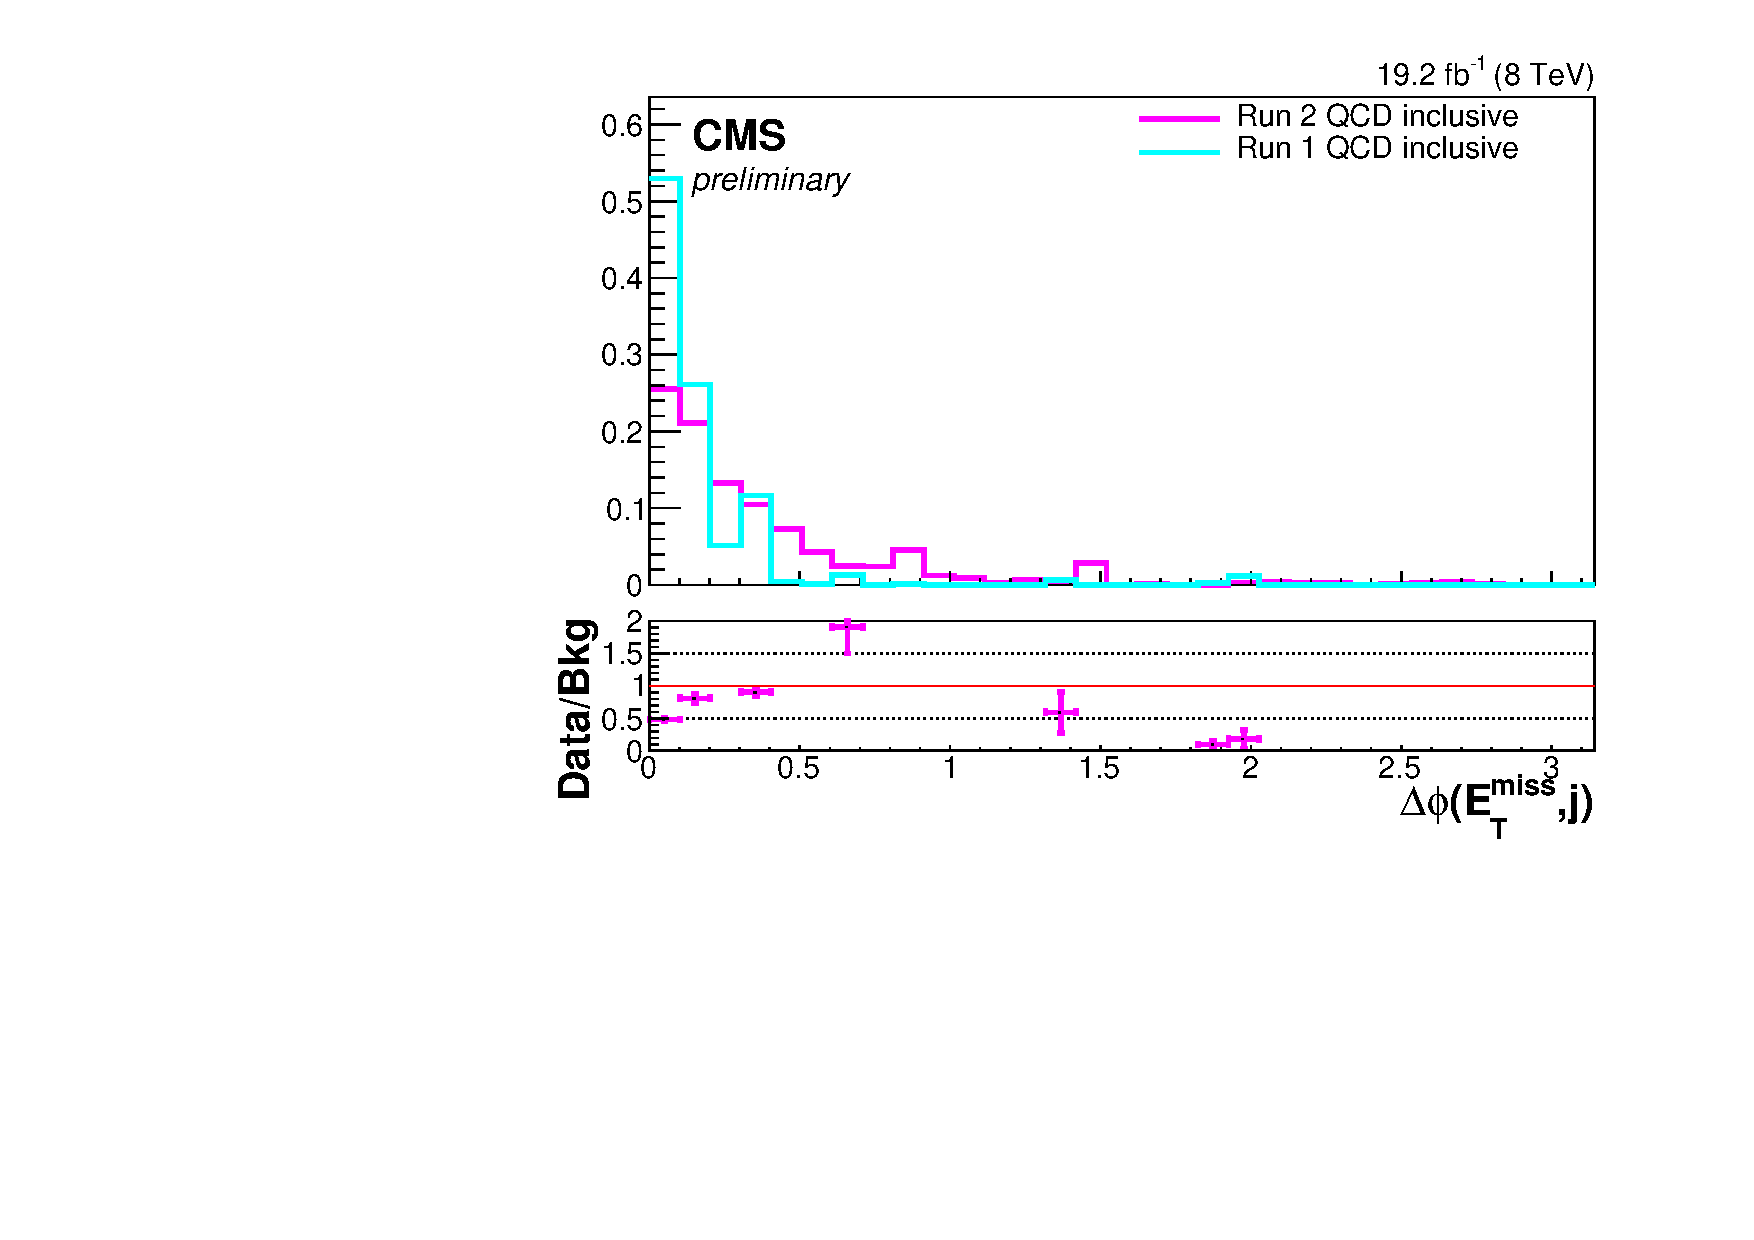
\includegraphics[width=.5\textwidth]{TalkPics/dmandqcd010615/qcdplots010615/nunu_norm_alljetsmetnomu_mindphi.pdf}
  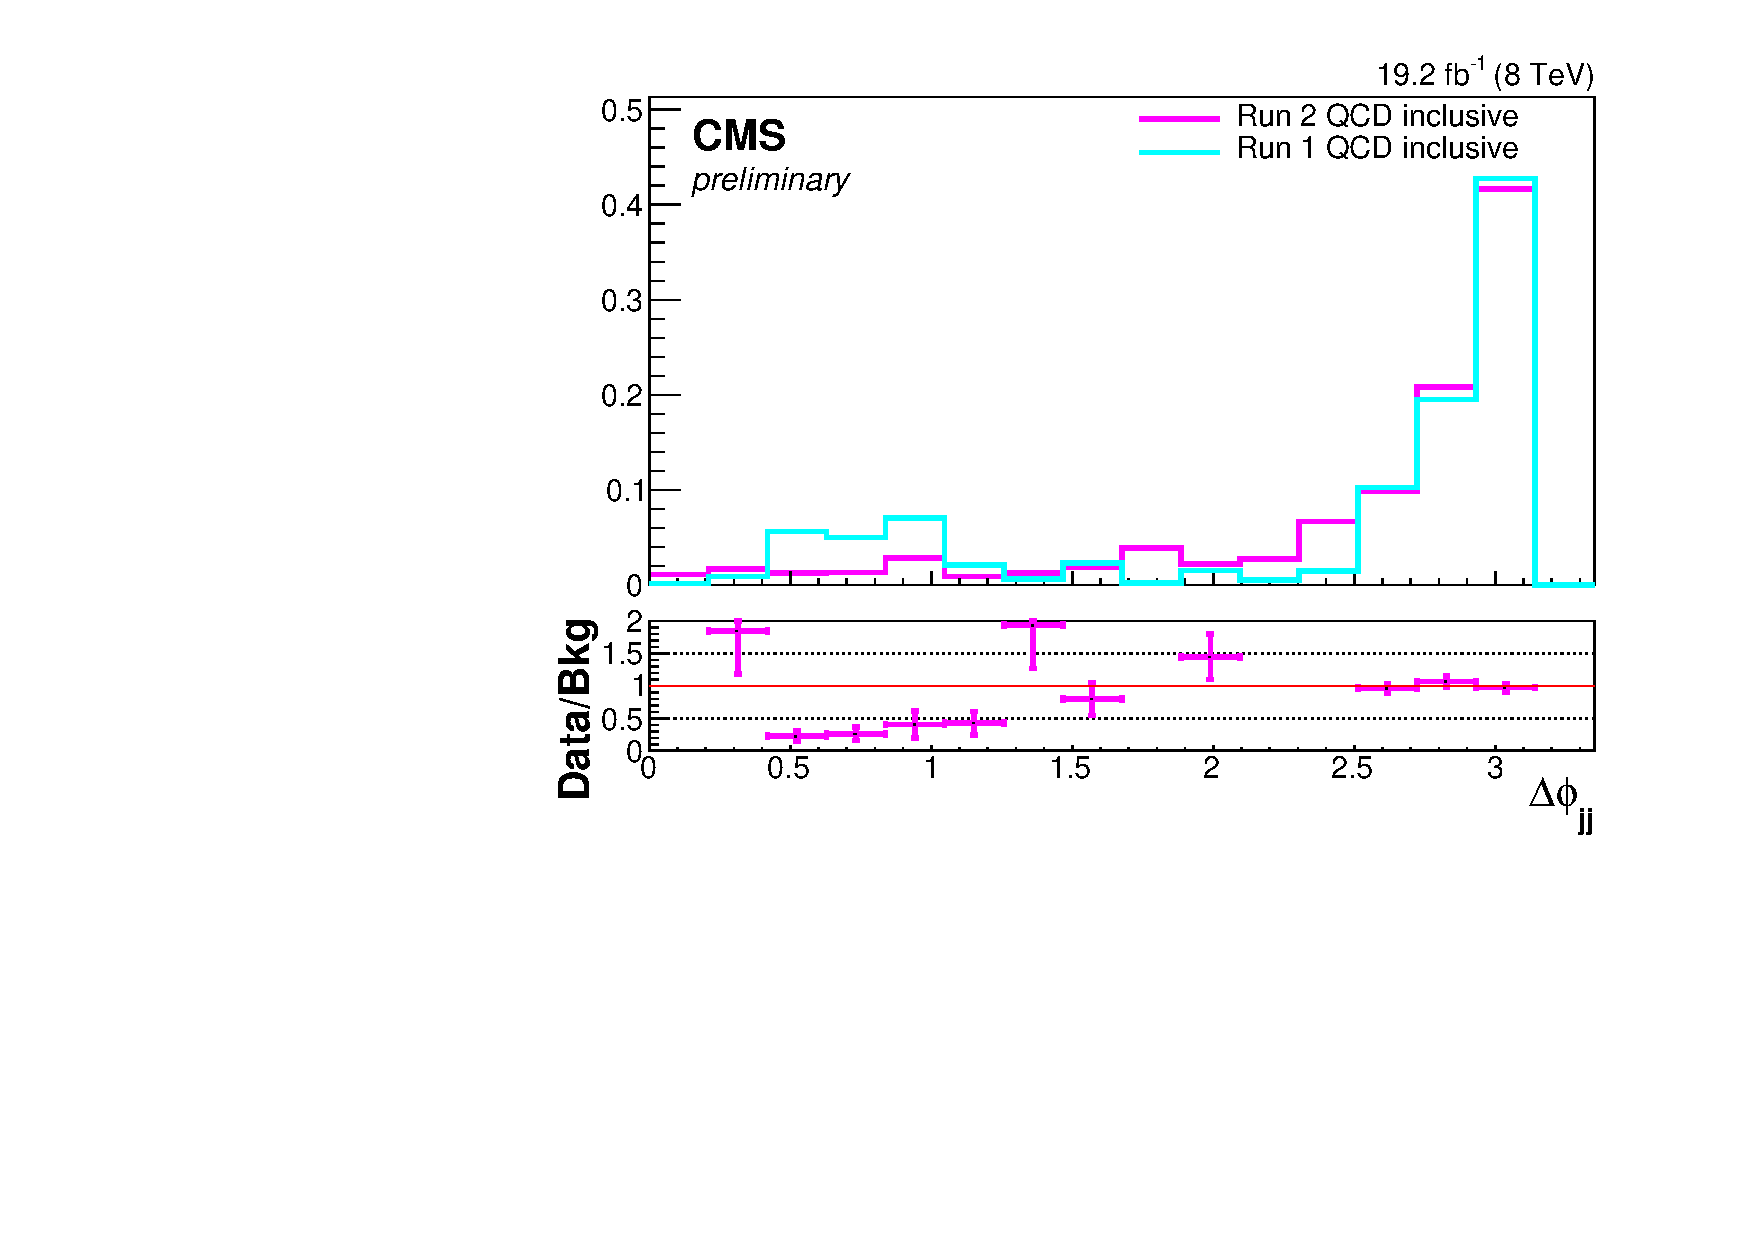
\includegraphics[width=.5\textwidth]{TalkPics/dmandqcd010615/qcdplots010615/nunu_norm_dijet_dphi.pdf}
  \begin{block}{}
    \begin{itemize}
    \item Both similar but limited by low stats
    \end{itemize}
  \end{block}
\end{frame}

\begin{frame}
  \frametitle{Signal comparison: run 1 vs run 2: dijet variables}
  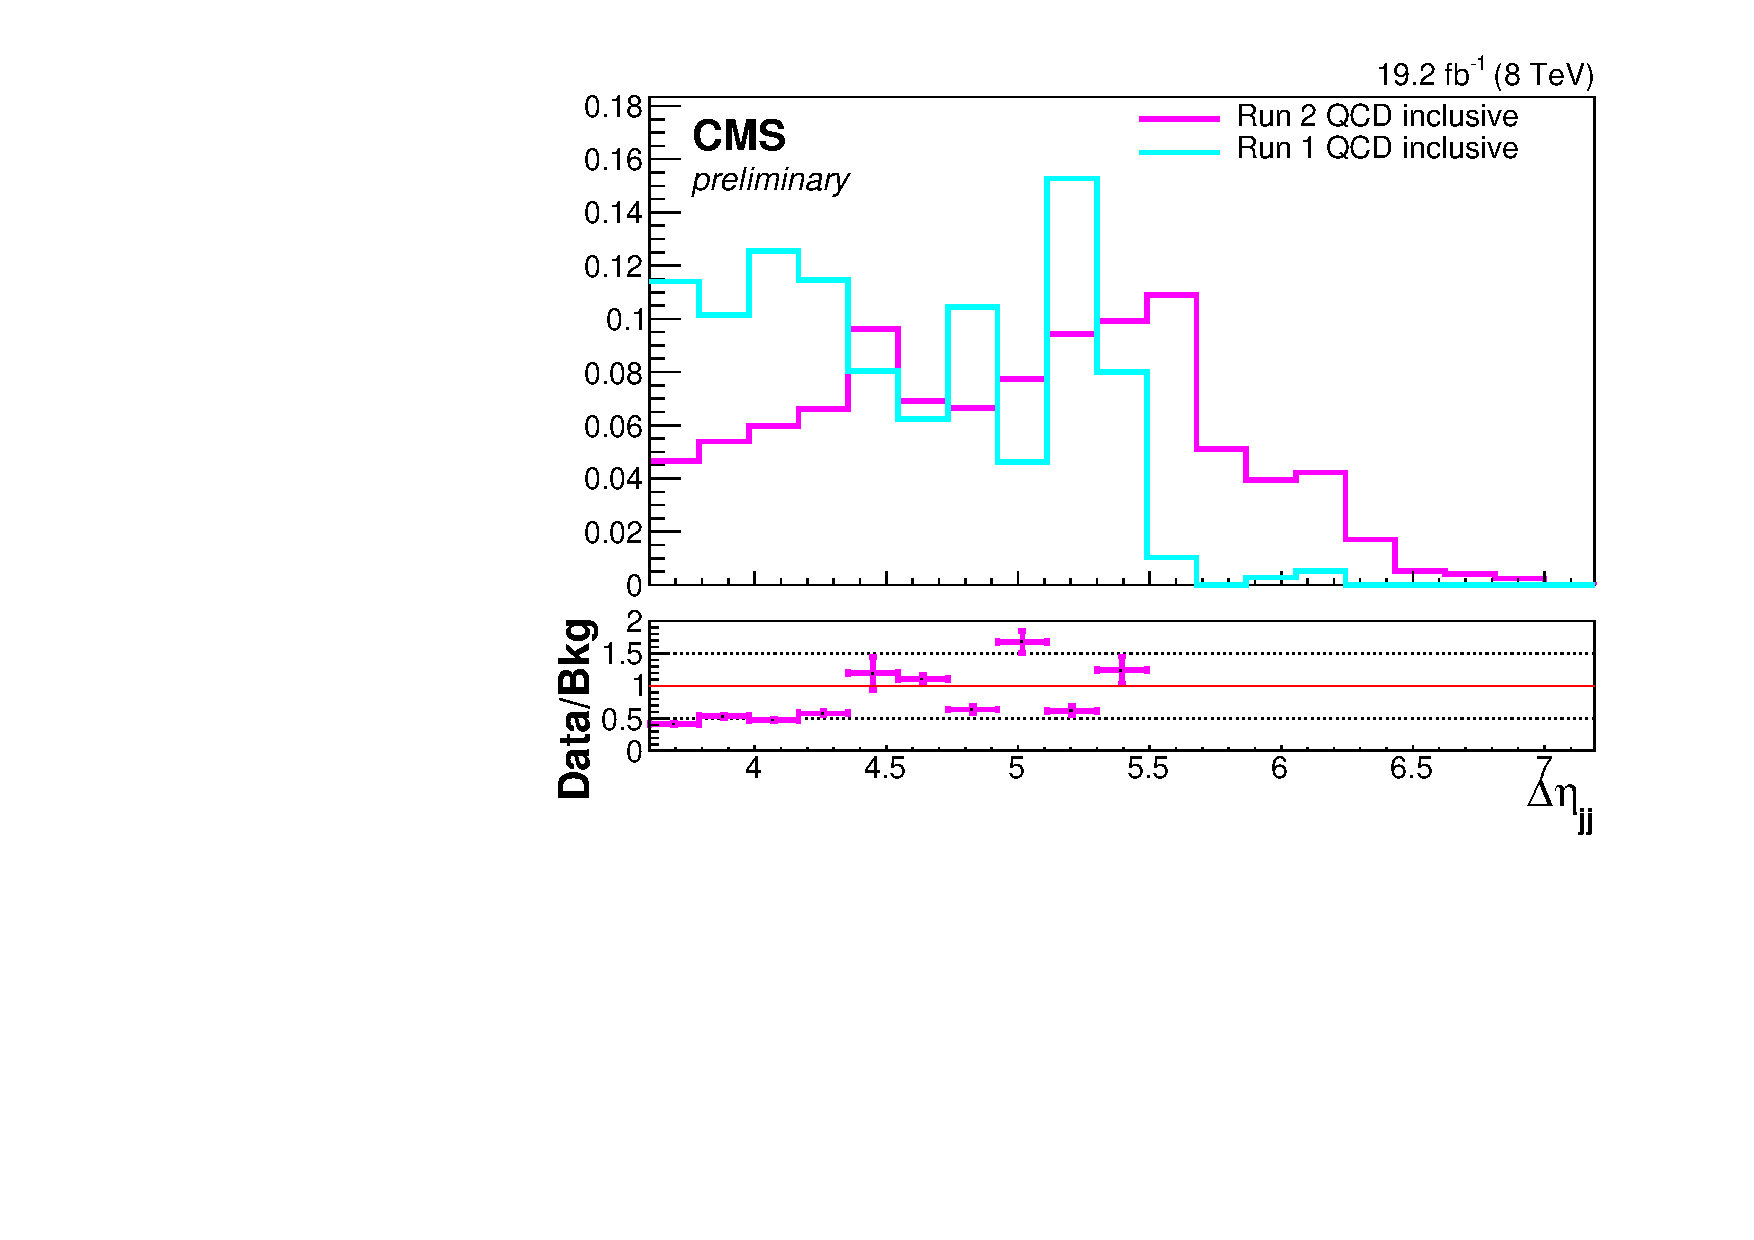
\includegraphics[width=.5\textwidth]{TalkPics/dmandqcd010615/qcdplots010615/nunu_norm_dijet_deta.pdf}
  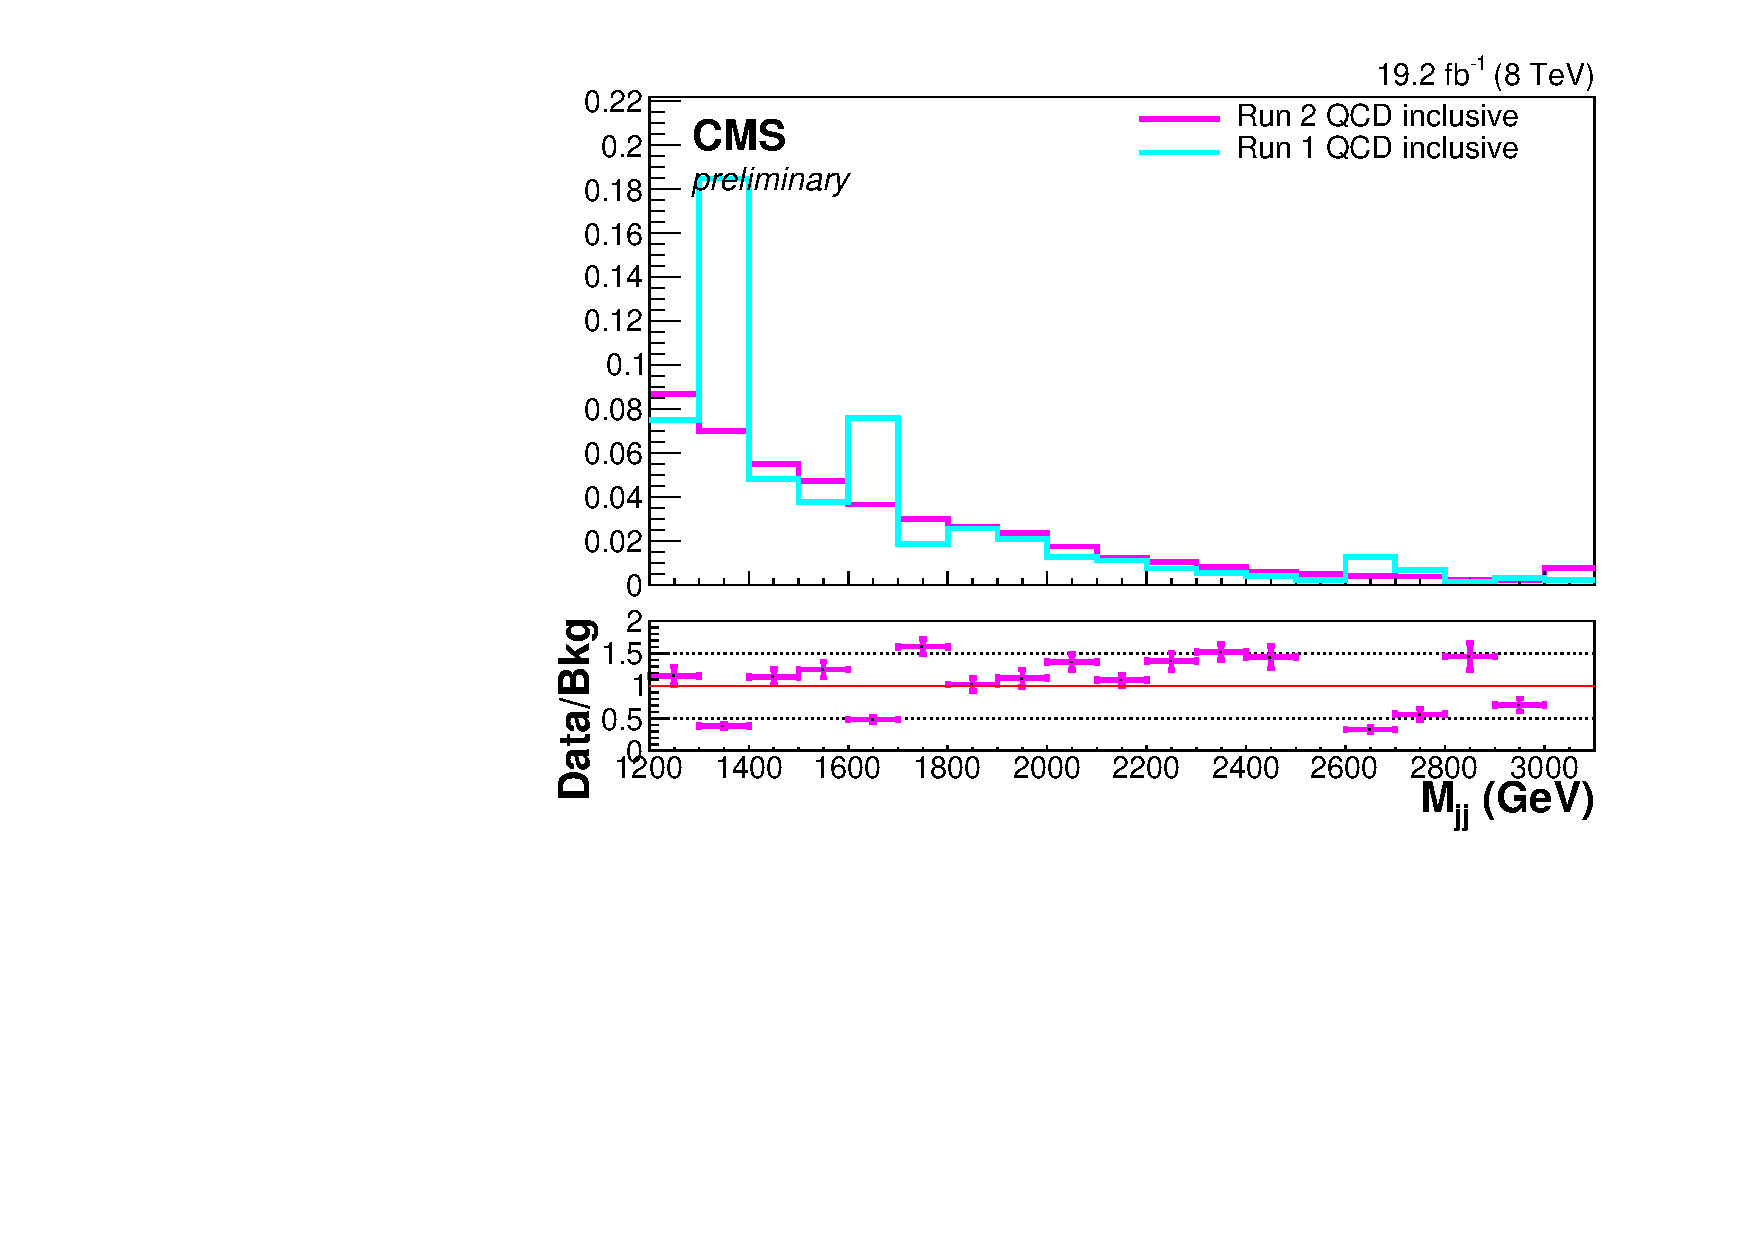
\includegraphics[width=.5\textwidth]{TalkPics/dmandqcd010615/qcdplots010615/nunu_norm_dijet_M.pdf}
   \begin{block}{}
     \begin{itemize}
     \item $\Delta\eta_{jj}$ larger for run 2: could be due to HF 
     \item $M_{jj}$ similar
     \end{itemize}
   \end{block}
\end{frame}

\begin{frame}
  \frametitle{Signal comparison: run 1 vs run 2: N jets}
  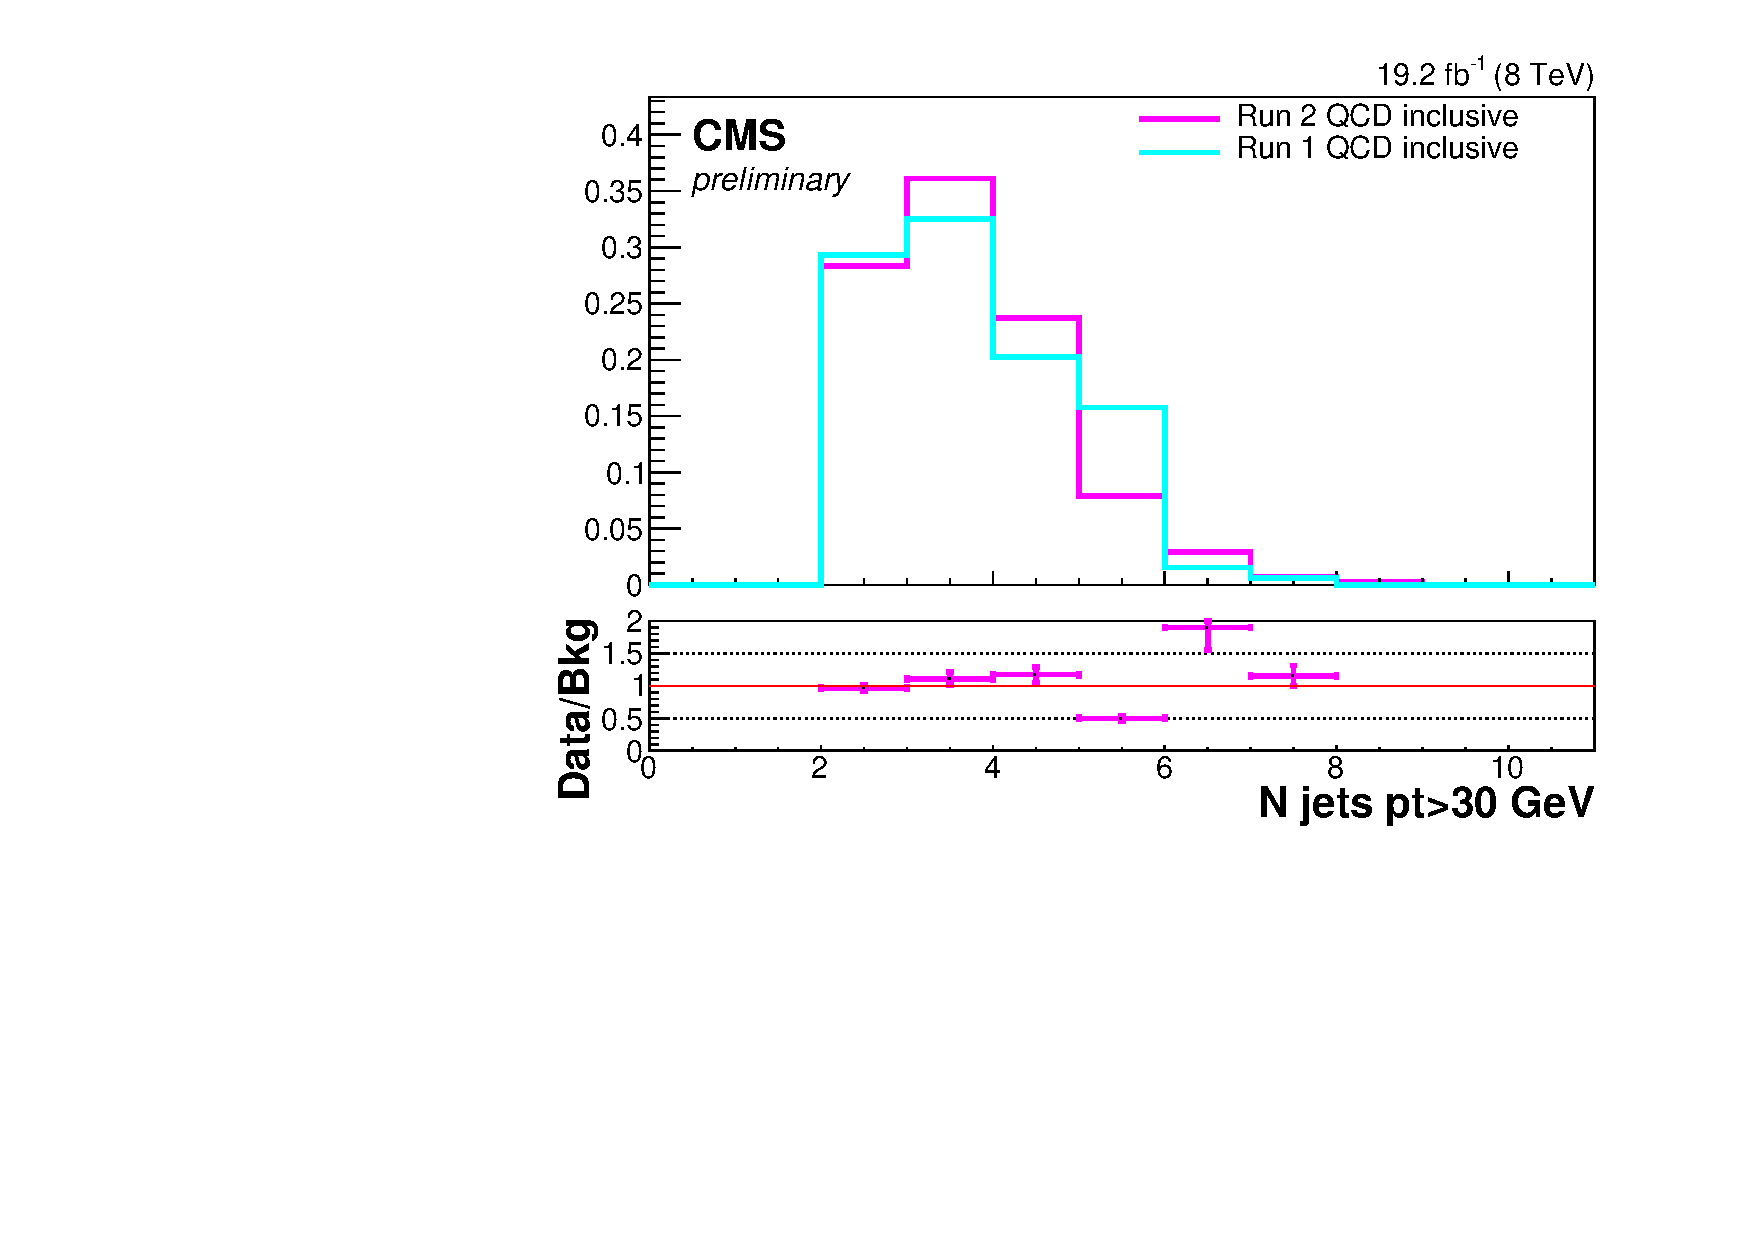
\includegraphics[width=.5\textwidth]{TalkPics/dmandqcd010615/qcdplots010615/nunu_norm_n_jets_30.pdf}
  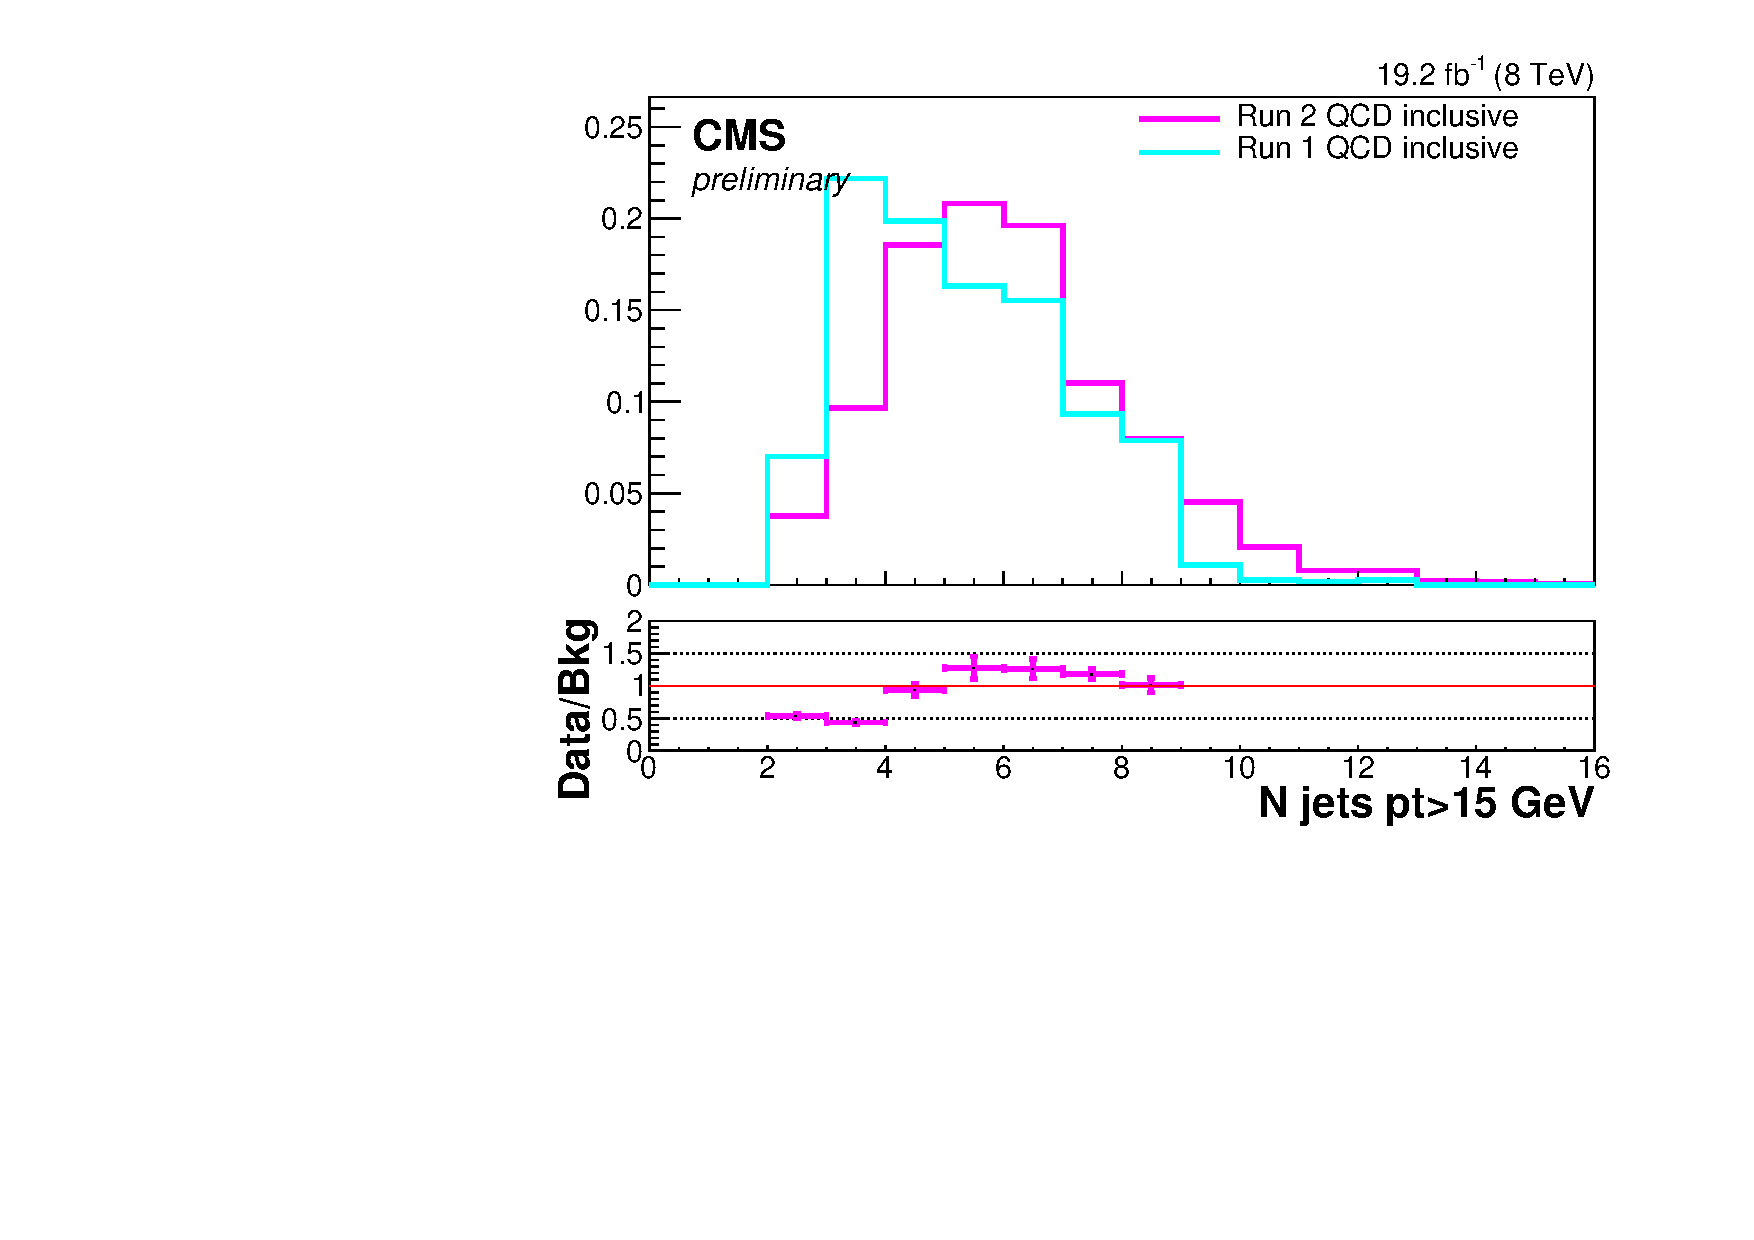
\includegraphics[width=.5\textwidth]{TalkPics/dmandqcd010615/qcdplots010615/nunu_norm_n_jets_15.pdf}
  \begin{block}{}
    \begin{itemize}
    \item Number of high pt jets similar, run 2 has more low pt jets
    \end{itemize}
  \end{block}
\end{frame}

\begin{frame}
  \frametitle{Higgs Portal DM interpretation - recap}
  \begin{block}{}
    \begin{itemize}
    \item For prompt paper made a DM limit using EFT described \href{http://www.sciencedirect.com/science/article/pii/S0370269312001037}{here}
    \item Since then the fermion line has been found to be invalid
    \item Other two lines should still be ok: I will double check this
    \end{itemize}
  \end{block}
  \centering
  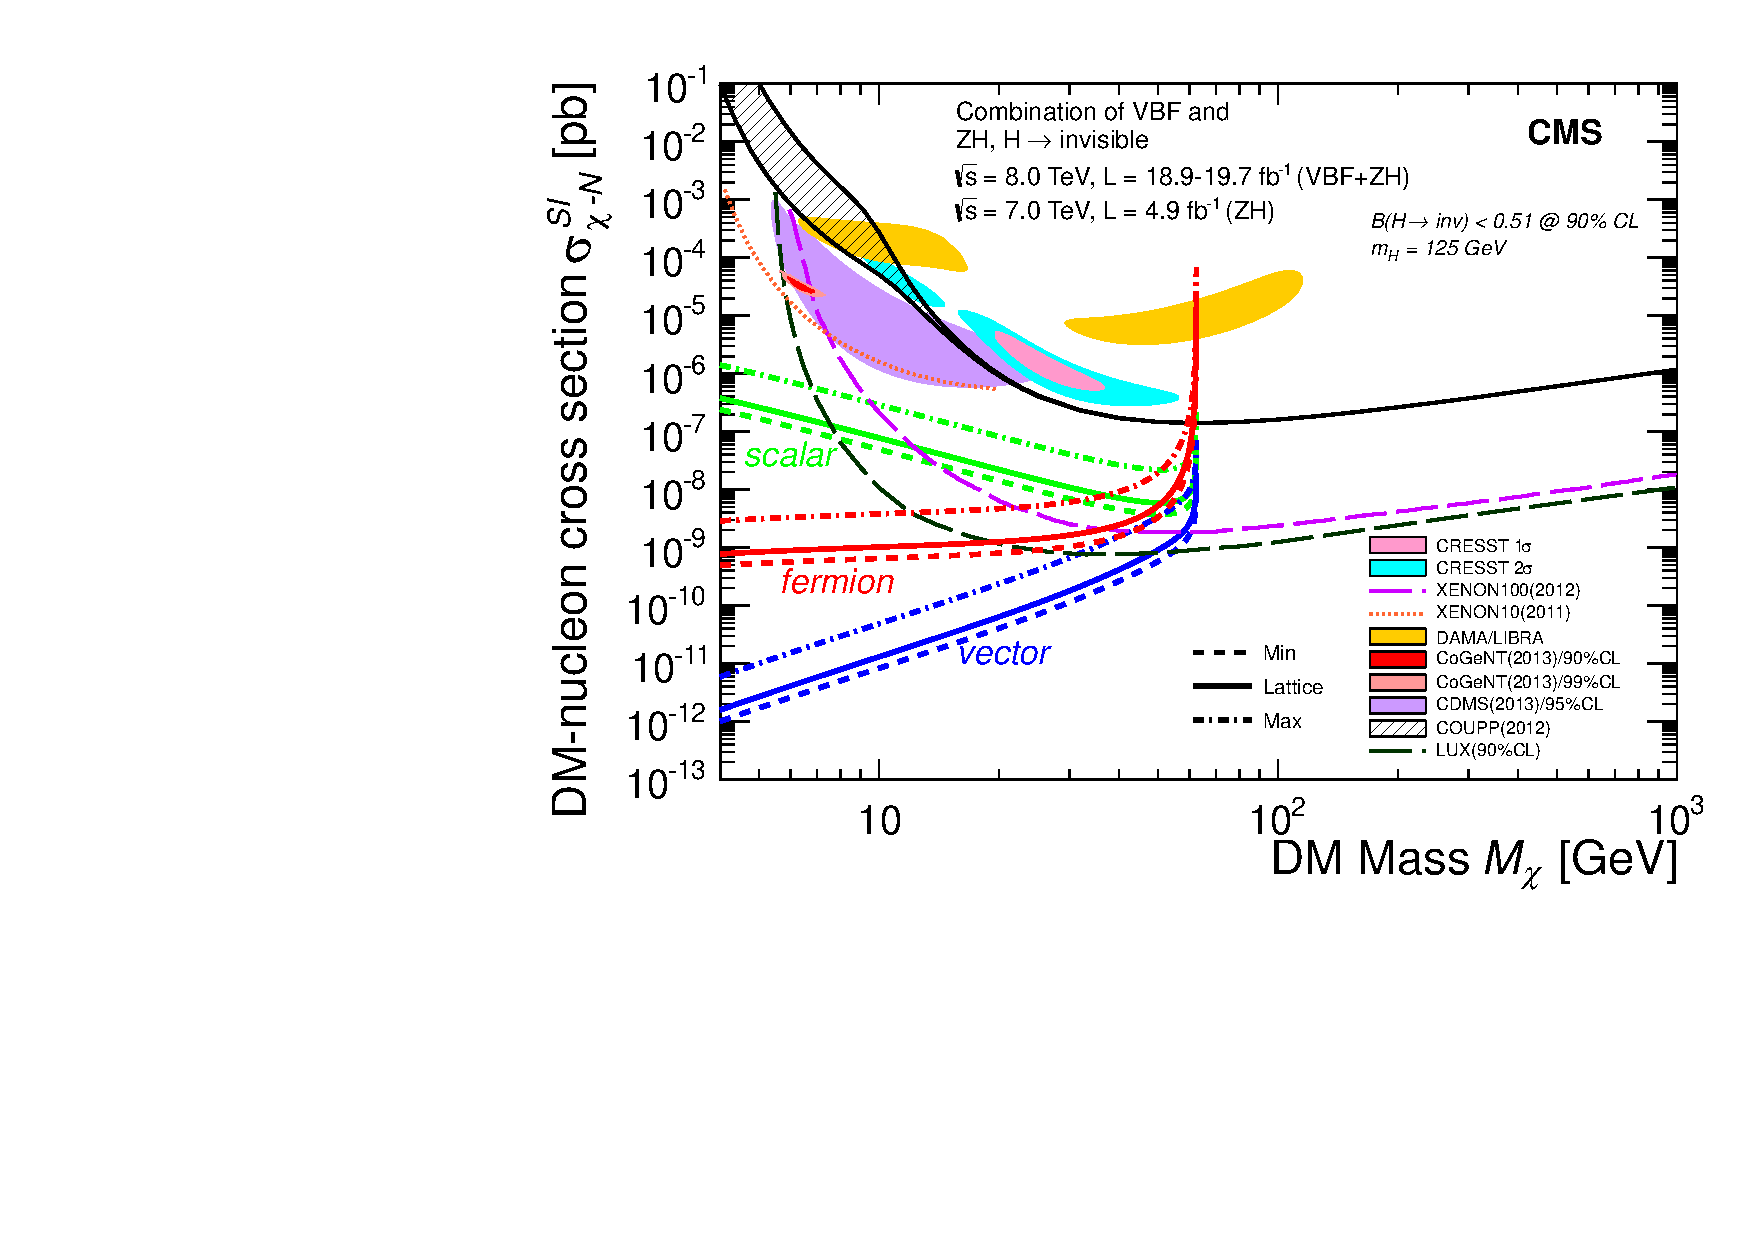
\includegraphics[width=.5\textwidth]{TalkPics/dmandqcd010615/promptdmnucleonlimit.pdf}
\end{frame}

\begin{frame}
  \frametitle{Higgs Portal DM interpretation - update}
  \begin{block}{}
    \begin{itemize}
    \item Used direct detection data from \href{dmtools.brown.edu:8080}{Brown DM tools}
    \item Use 90\% CL observed limit from HIG14038 result: 0.4048
    \item Left plot has three values of fN as in paper
    \item Right plot is prompt (dashed) vs parked plus EXO (solid)
    \end{itemize}
  \end{block}
  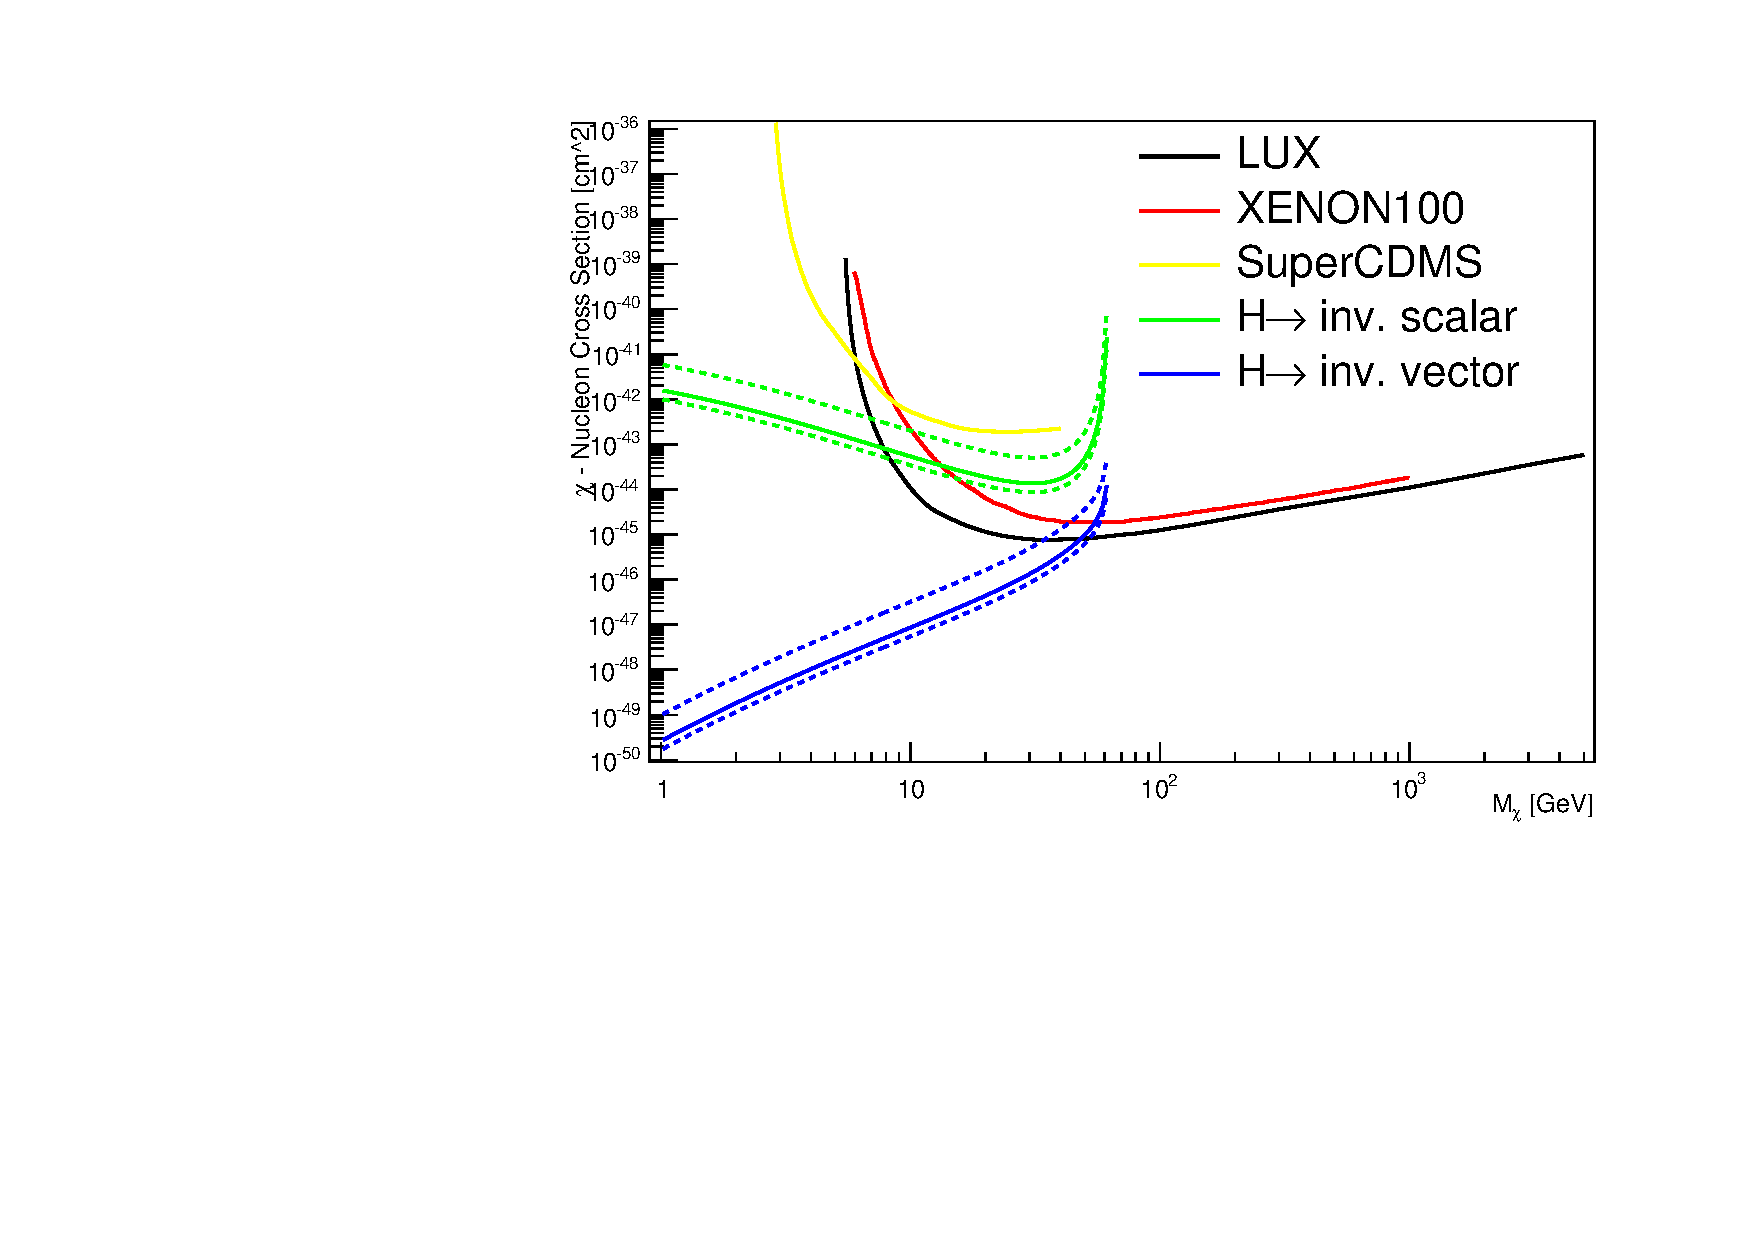
\includegraphics[width=.5\textwidth]{TalkPics/dmandqcd010615/DMplot.pdf}
  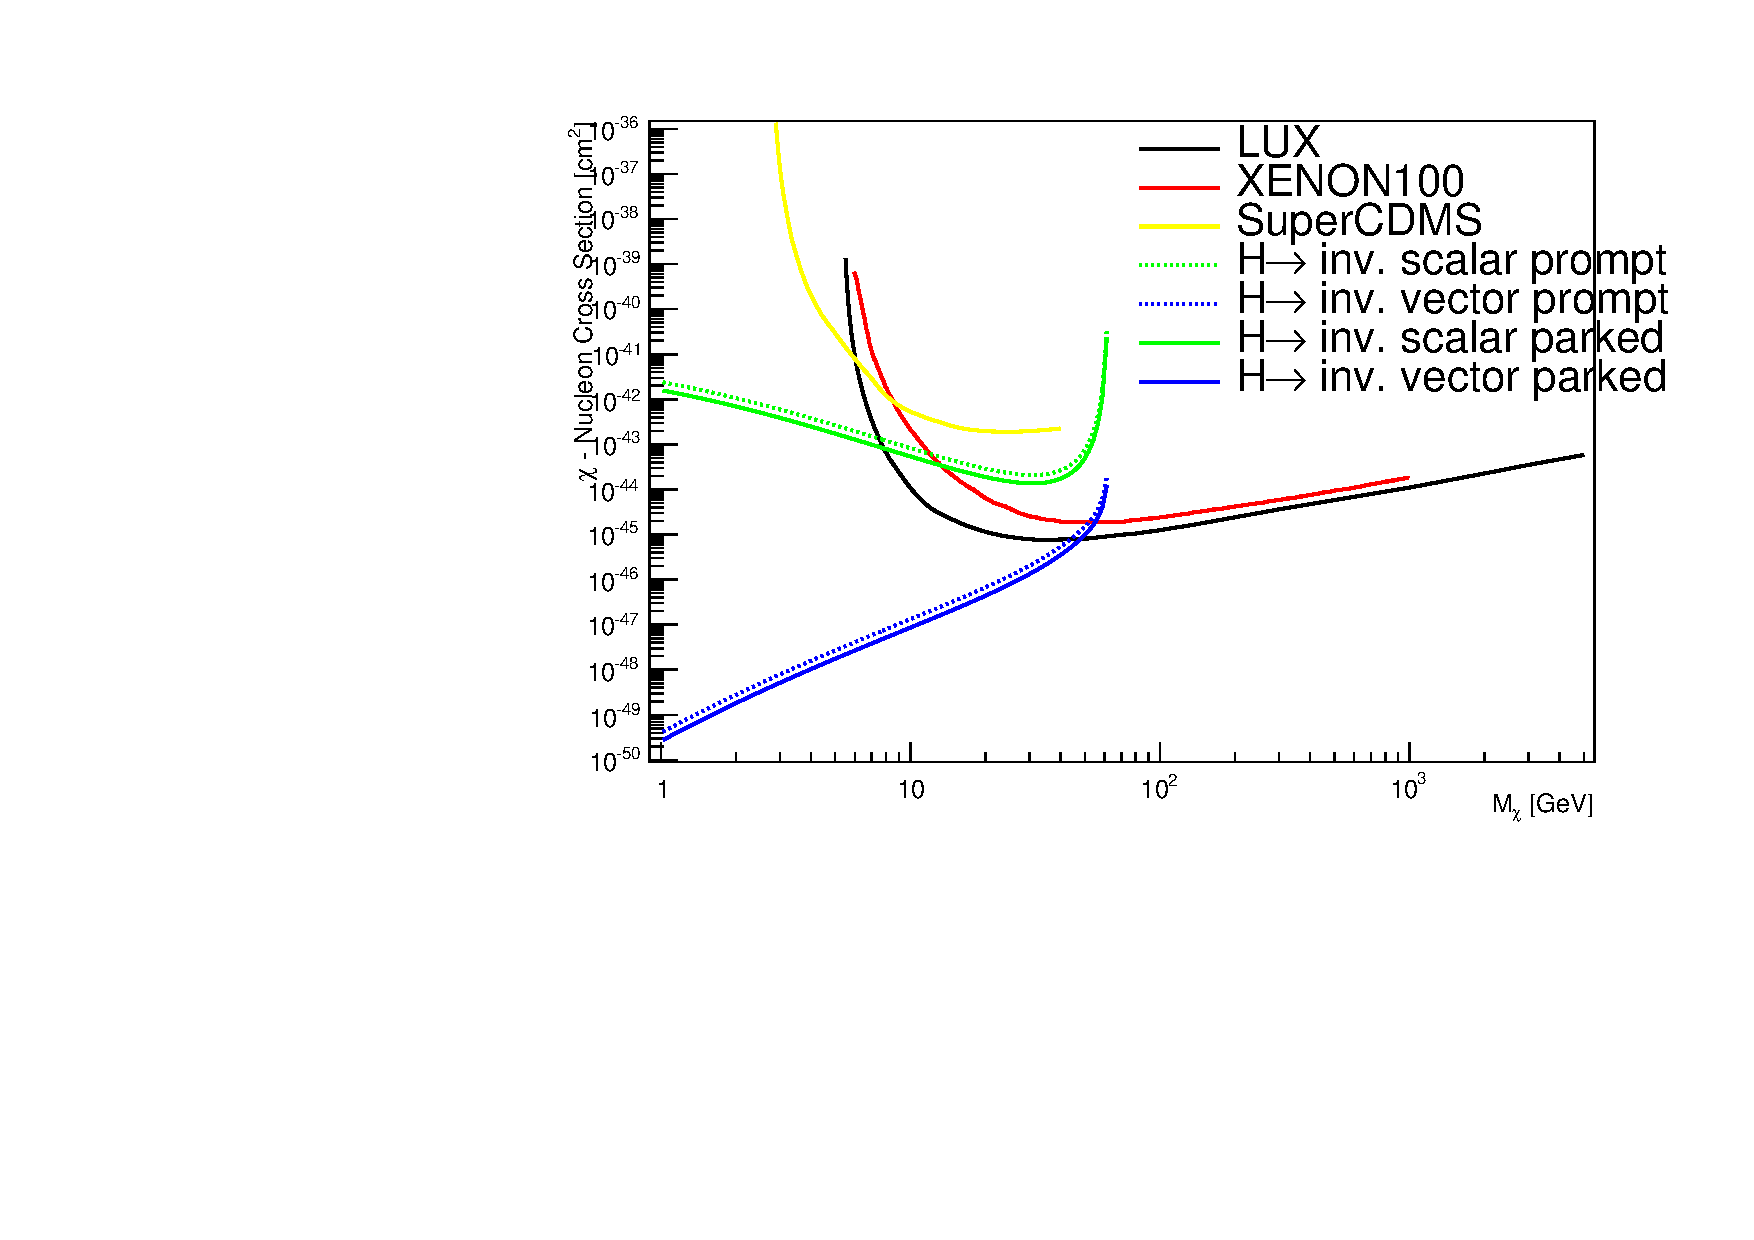
\includegraphics[width=.5\textwidth]{TalkPics/dmandqcd010615/DMplotpromptvsparked.pdf}
\end{frame}

\begin{frame}
 \frametitle{Combination with EXO result}
  \begin{block}{}
    \begin{itemize}
    \item Working with Nick to combine VBF, ZH and EXO result
    \item At first there was $\sim$ 0.02 difference in expected limit between our results
    \item My numbers: expected) 0.2998
    \item Two differences identified:
    \item Nick using $\Delta$LL$=4$, I was using 95\% C.L.
    \item[-] On both using 95\% C.L. difference went to 0.004
    \item I was running the 7 TeV Z(ll)H cards and Nick wasn't
    \item[-] When I take out the 7 TeV cards this difference goes away
    \end{itemize}
  \end{block}
\end{frame}

\begin{frame}
  \label{lastframe}
  \begin{block}{Summary}
    \begin{itemize}
    \item First look at QCD samples:
    \item[-] Limited stats especially in run 1 so hard to draw conclusions
    \item[-] Also neither set models fake met so we will still need Joao's samples
    \item DM plot remade:
    \item[-] Double checking validity of scalar and vector lines
    \item[-] Can add other experiments if desired
    \item Combination with EXO:
    \item[-] Synchronising with Nick
    \item[-] PAS waiting on approval of EXO result
    \end{itemize}
  \end{block}
\end{frame}

\begin{frame}
  \frametitle{Backup}
\end{frame}

\end{fmffile}
\end{document}
